\section{Detekcja twarzy}
W rozdziale tym opisano testy przeprowadzone w celu oceniania skuteczności działania wybranych detektorów twarzy. Podjęto decyzję o wykonaniu kilku zdjęć przedstawiających twarz w różnych pozycjach, częściowo zasłoniętą oraz w zmiennym oświetleniu. Wizualizację wyników przeprowadzonych testów zawarto w tabeli \ref{tab:porownanie_detektorow}.
\begin{longtable}{|c|c|c|c|c|c|} 
\hline
  		& \bfseries Wejście & \bfseries Haar & \bfseries Dnn & \bfseries Azure \\
  		\hline
  		1&		\begin{minipage}{.2\textwidth}
      	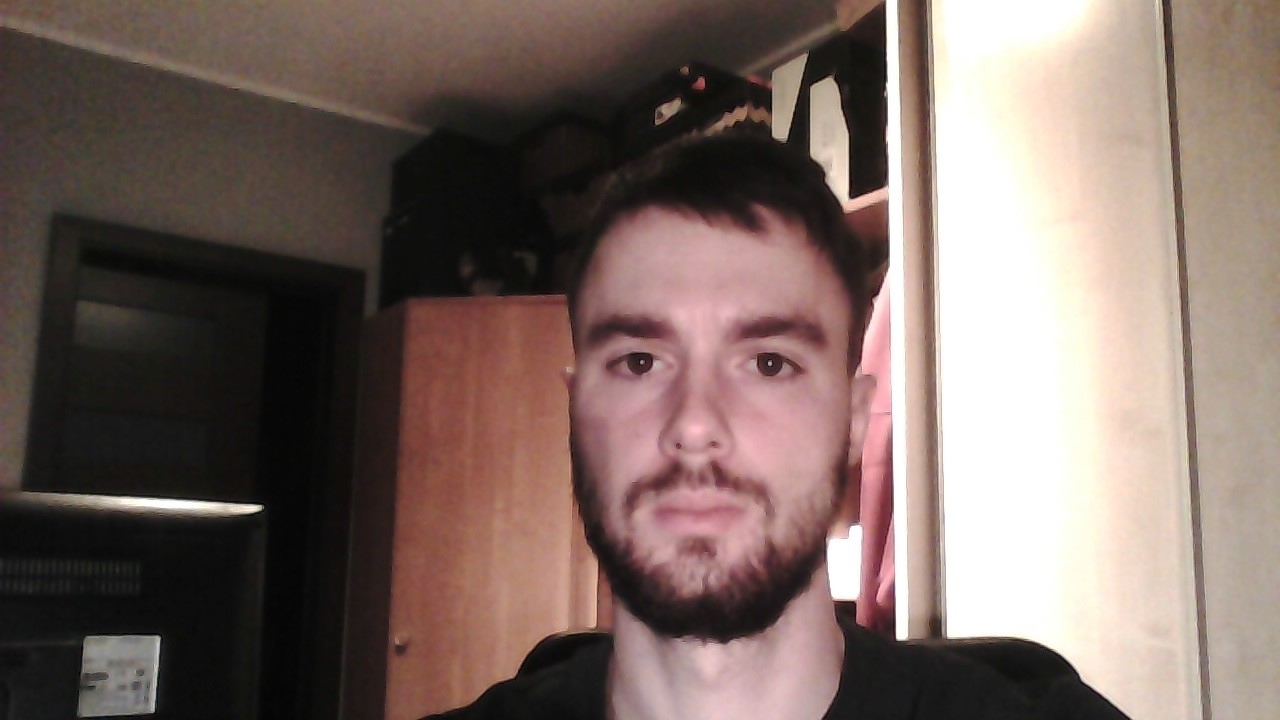
\includegraphics[width=\linewidth, height=20mm]{detekcja/3_input.jpg}
    	\end{minipage}
		& 
		\begin{minipage}{.2\textwidth}
      	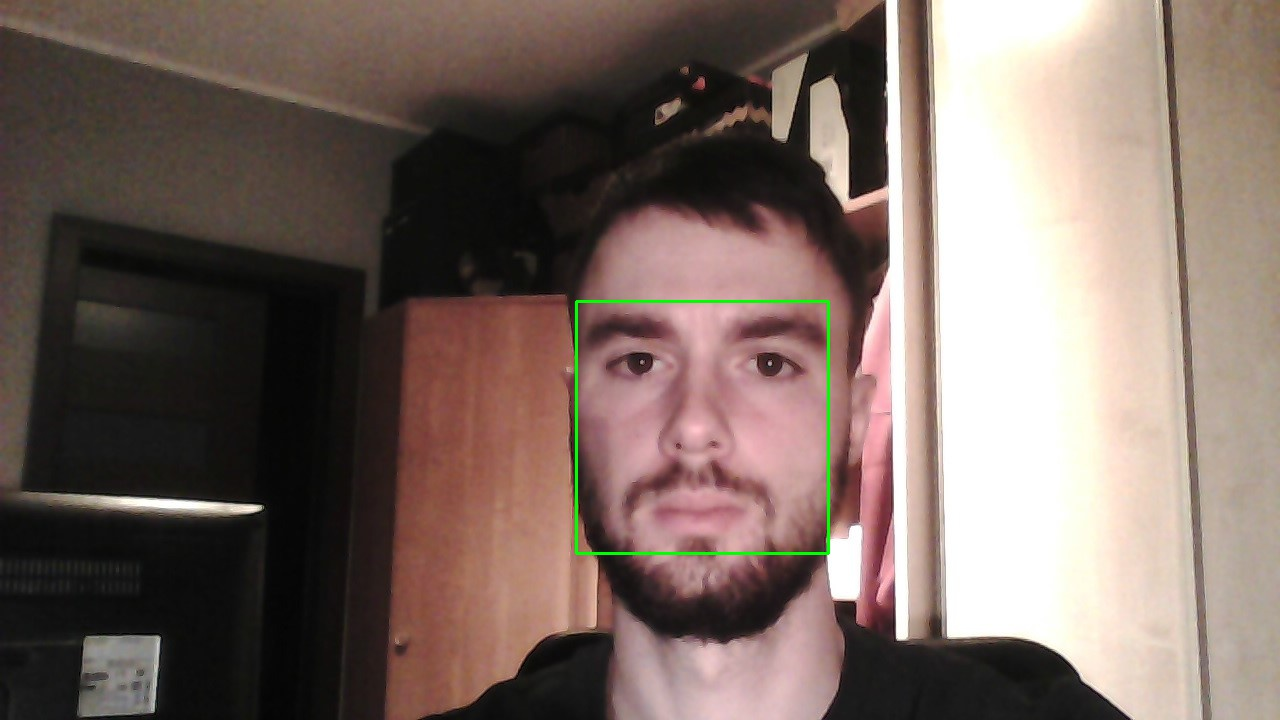
\includegraphics[width=\linewidth, height=20mm]{detekcja/3_haar.jpg}
    	\end{minipage}
		& 
		\begin{minipage}{.2\textwidth}
      	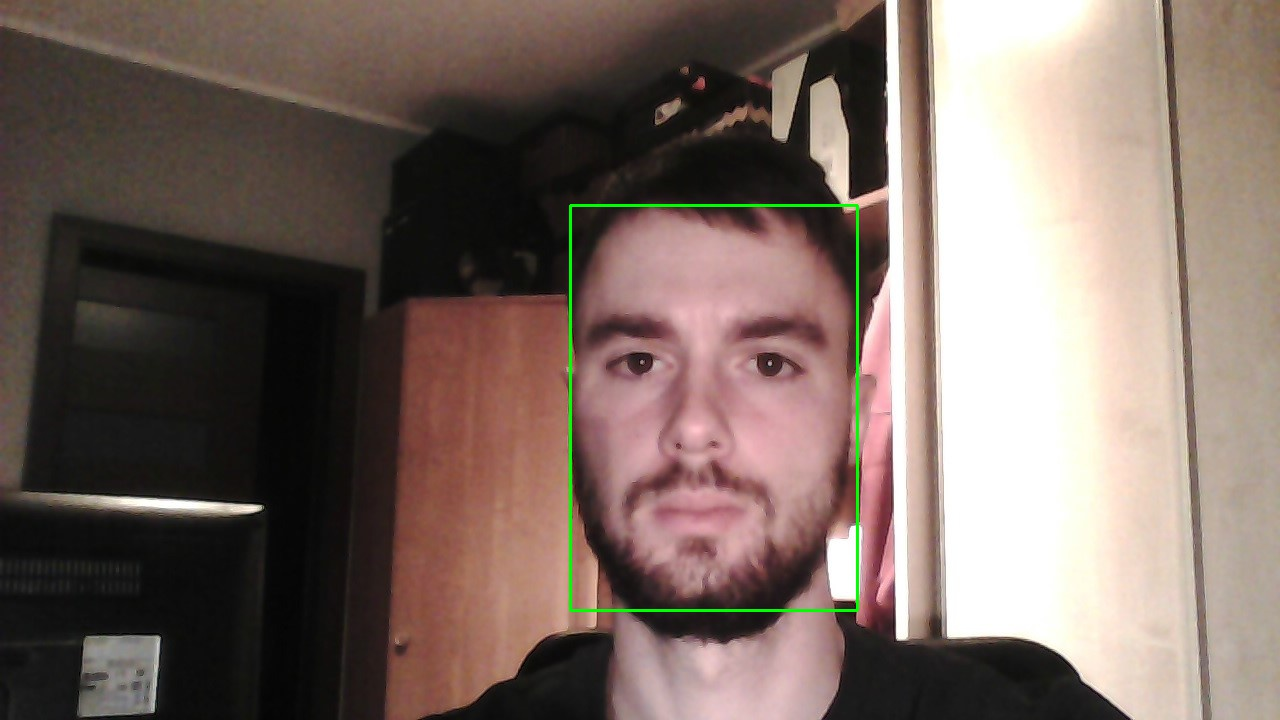
\includegraphics[width=\linewidth, height=20mm]{detekcja/3_dnn.jpg}
    	\end{minipage}
		& 
		\begin{minipage}{.2\textwidth}
      	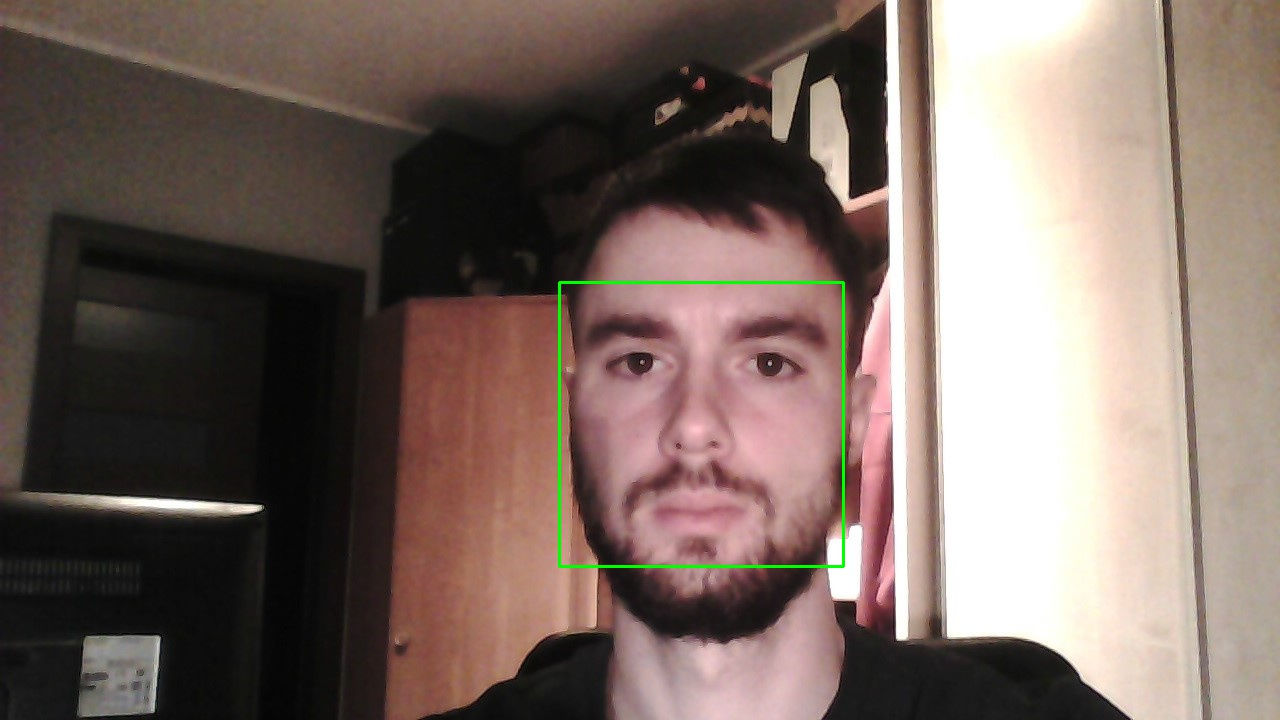
\includegraphics[width=\linewidth, height=20mm]{detekcja/3_azure.jpg}
    	\end{minipage}	
		\\
  		\hline
  		2&		\begin{minipage}{.2\textwidth}
      	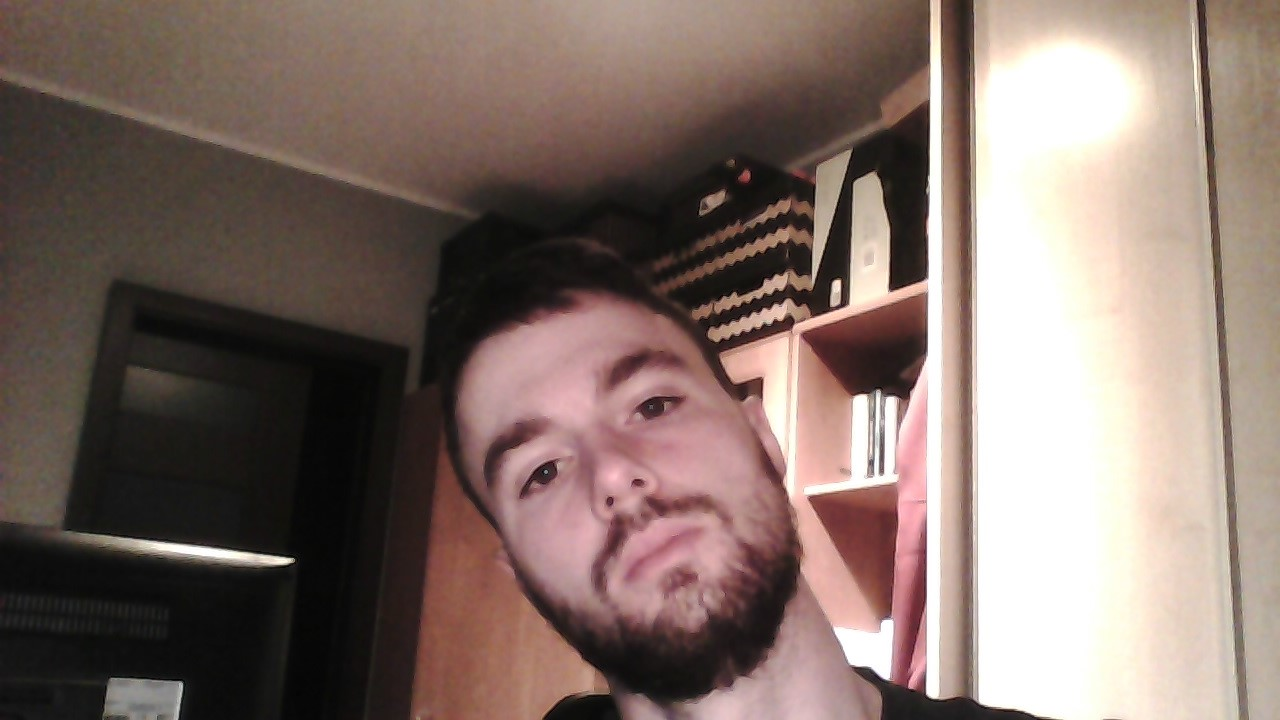
\includegraphics[width=\linewidth, height=20mm]{detekcja/4_input.jpg}
    	\end{minipage}
		& 
		\begin{minipage}{.2\textwidth}
      	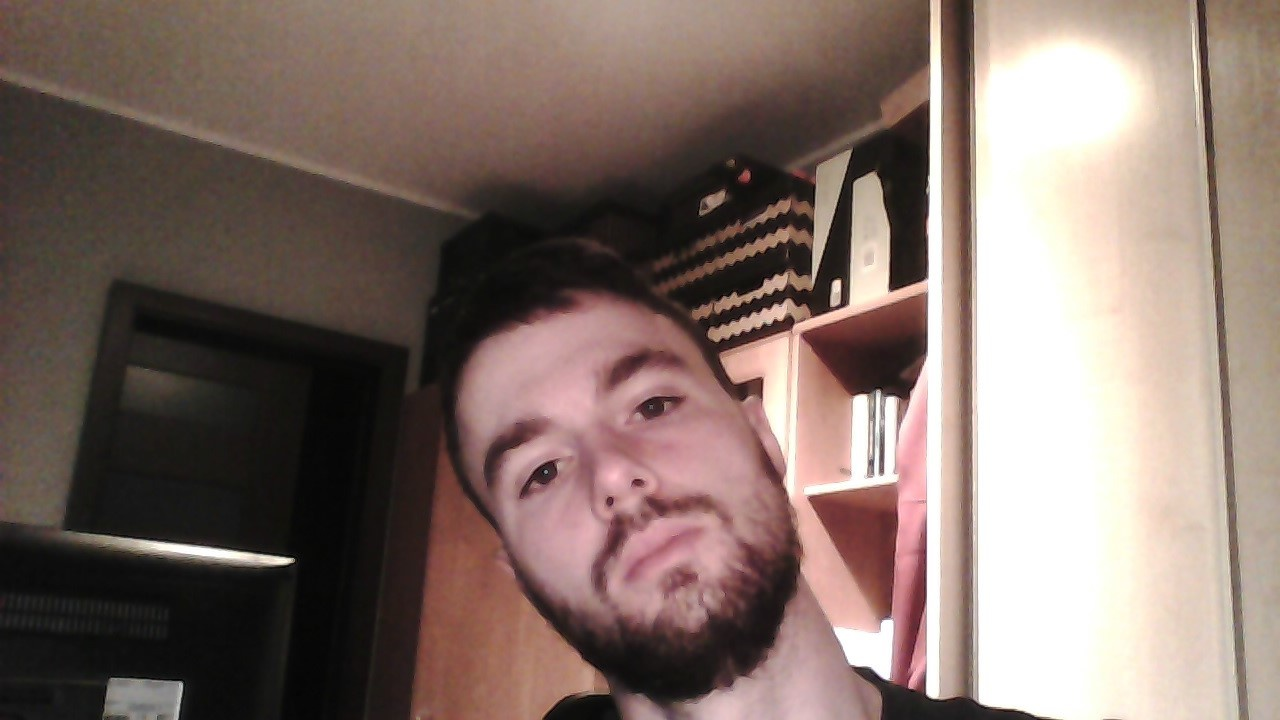
\includegraphics[width=\linewidth, height=20mm]{detekcja/4_haar.jpg}
    	\end{minipage}
		& 
		\begin{minipage}{.2\textwidth}
      	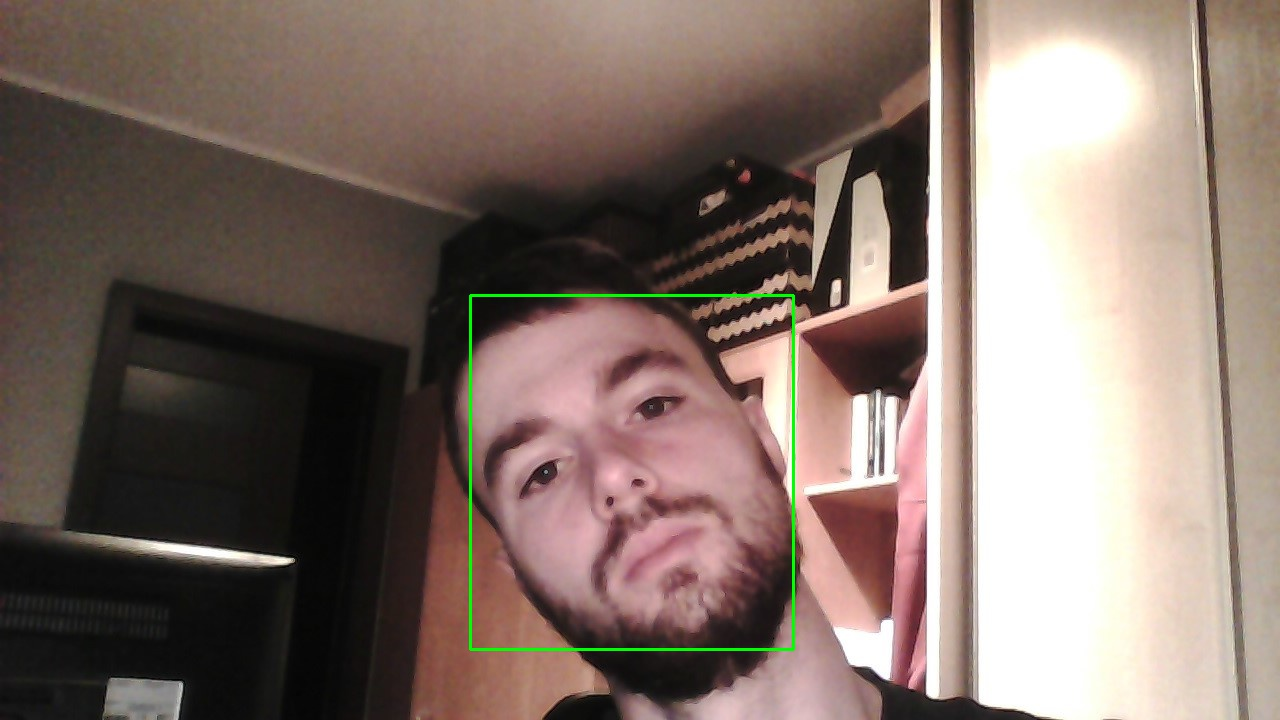
\includegraphics[width=\linewidth, height=20mm]{detekcja/4_dnn.jpg}
    	\end{minipage}
		& 
		\begin{minipage}{.2\textwidth}
      	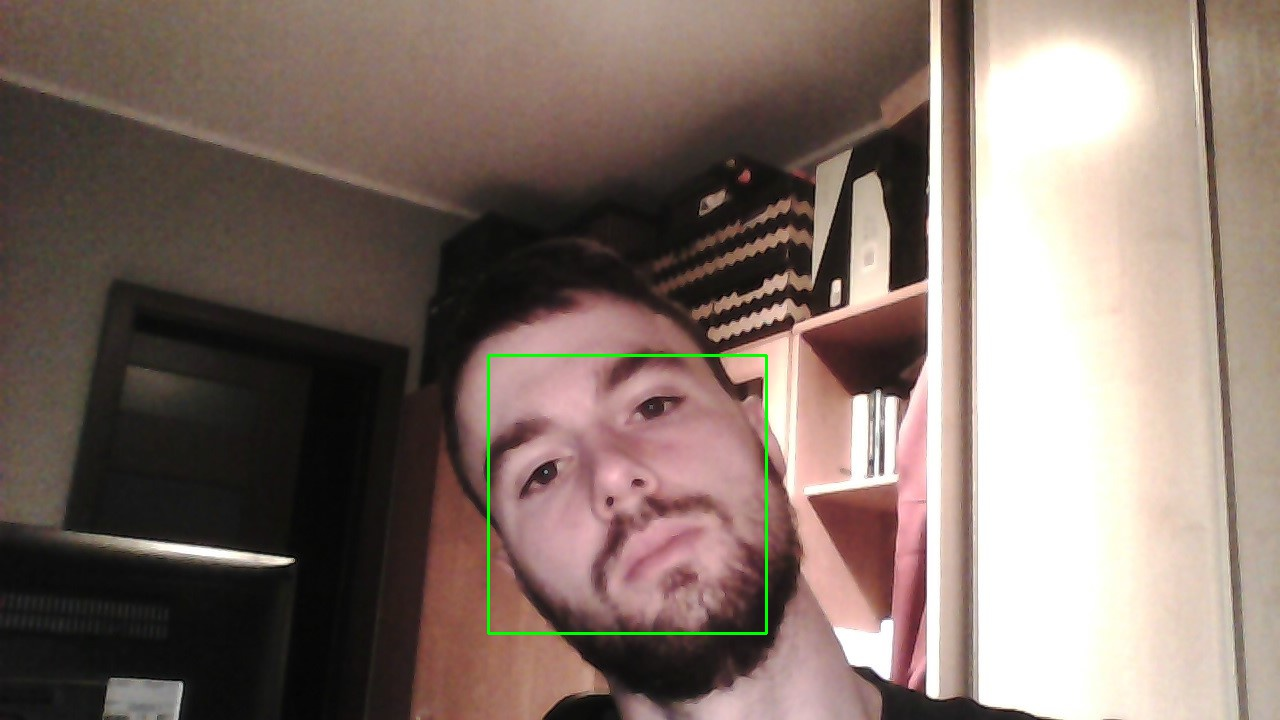
\includegraphics[width=\linewidth, height=20mm]{detekcja/4_azure.jpg}
    	\end{minipage}	
		\\
  		\hline
  		3& 		\begin{minipage}{.2\textwidth}
      	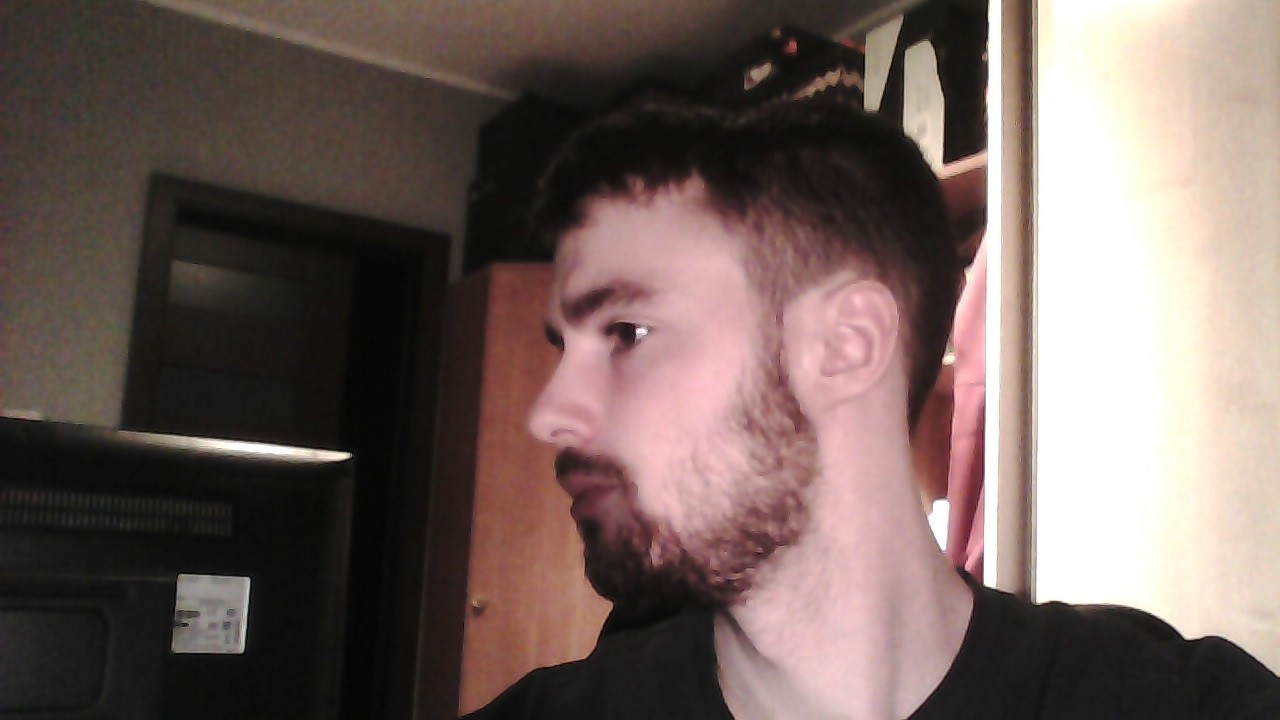
\includegraphics[width=\linewidth, height=20mm]{detekcja/5_input.jpg}
    	\end{minipage}
		& 
		\begin{minipage}{.2\textwidth}
      	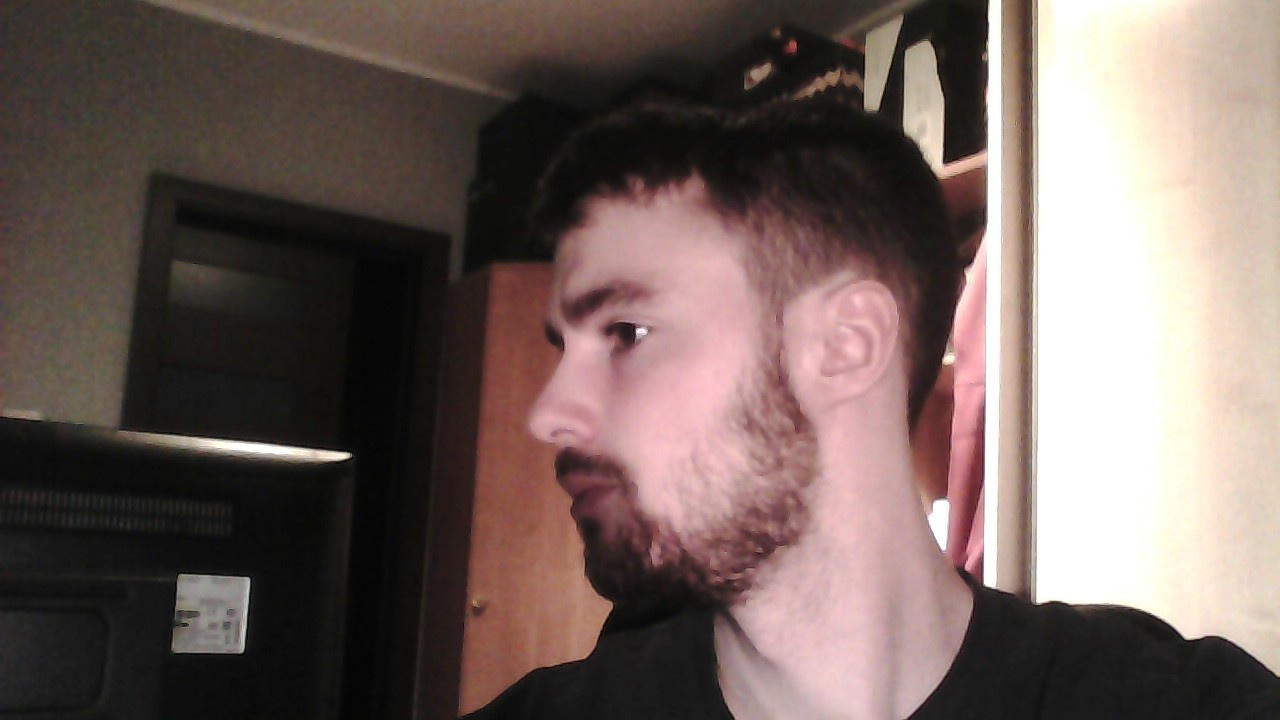
\includegraphics[width=\linewidth, height=20mm]{detekcja/5_haar.jpg}
    	\end{minipage}
		& 
		\begin{minipage}{.2\textwidth}
      	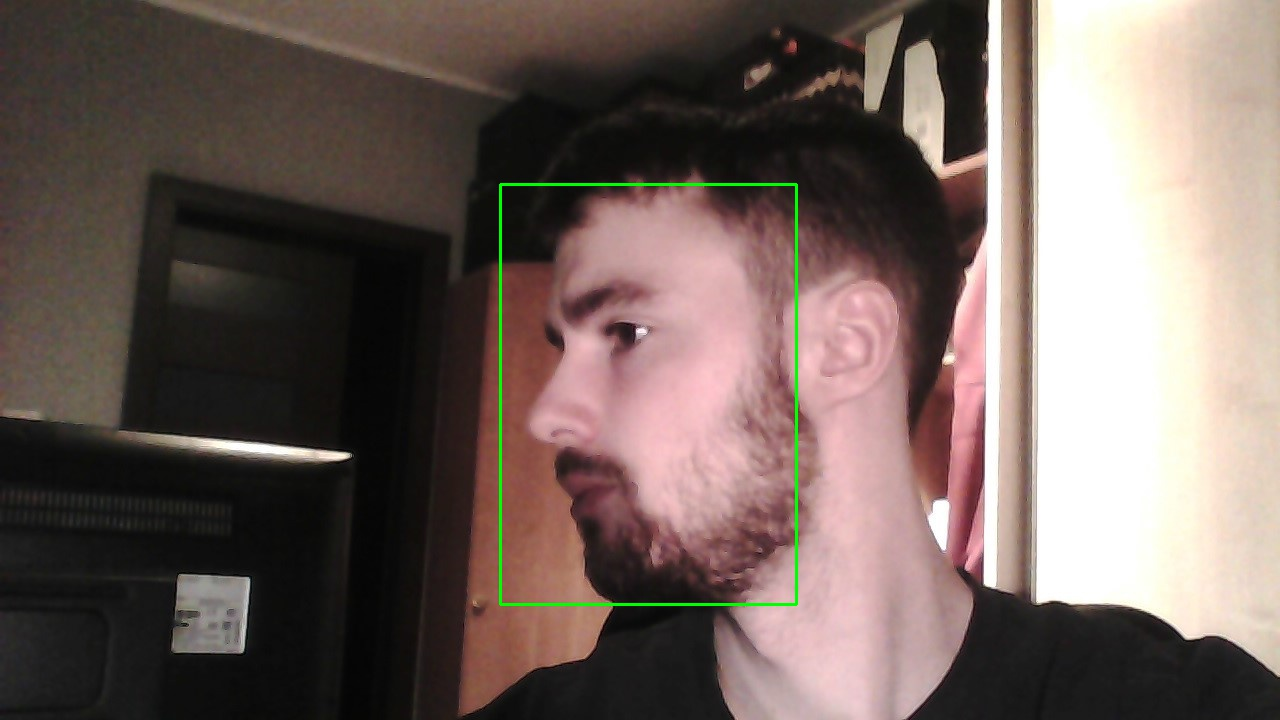
\includegraphics[width=\linewidth, height=20mm]{detekcja/5_dnn.jpg}
    	\end{minipage}
		& 
		\begin{minipage}{.2\textwidth}
      	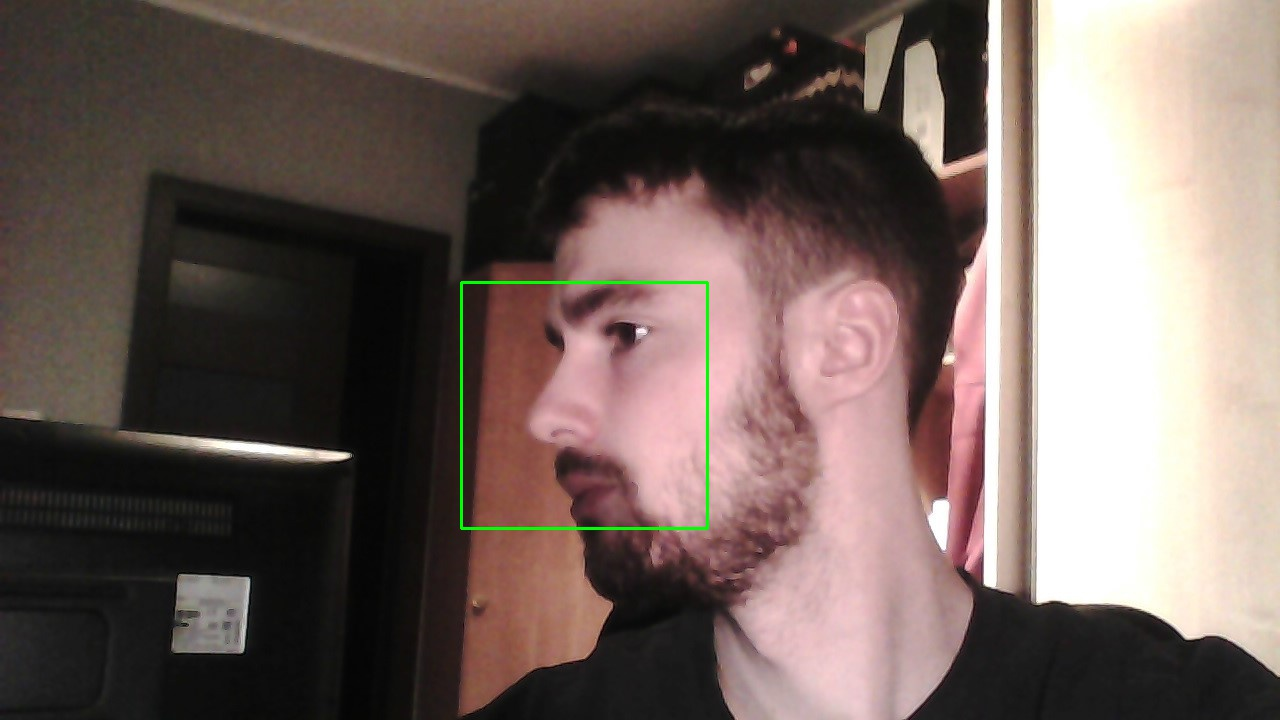
\includegraphics[width=\linewidth, height=20mm]{detekcja/5_azure.jpg}
    	\end{minipage}	
		\\
  		\hline
  		4&  		\begin{minipage}{.2\textwidth}
      	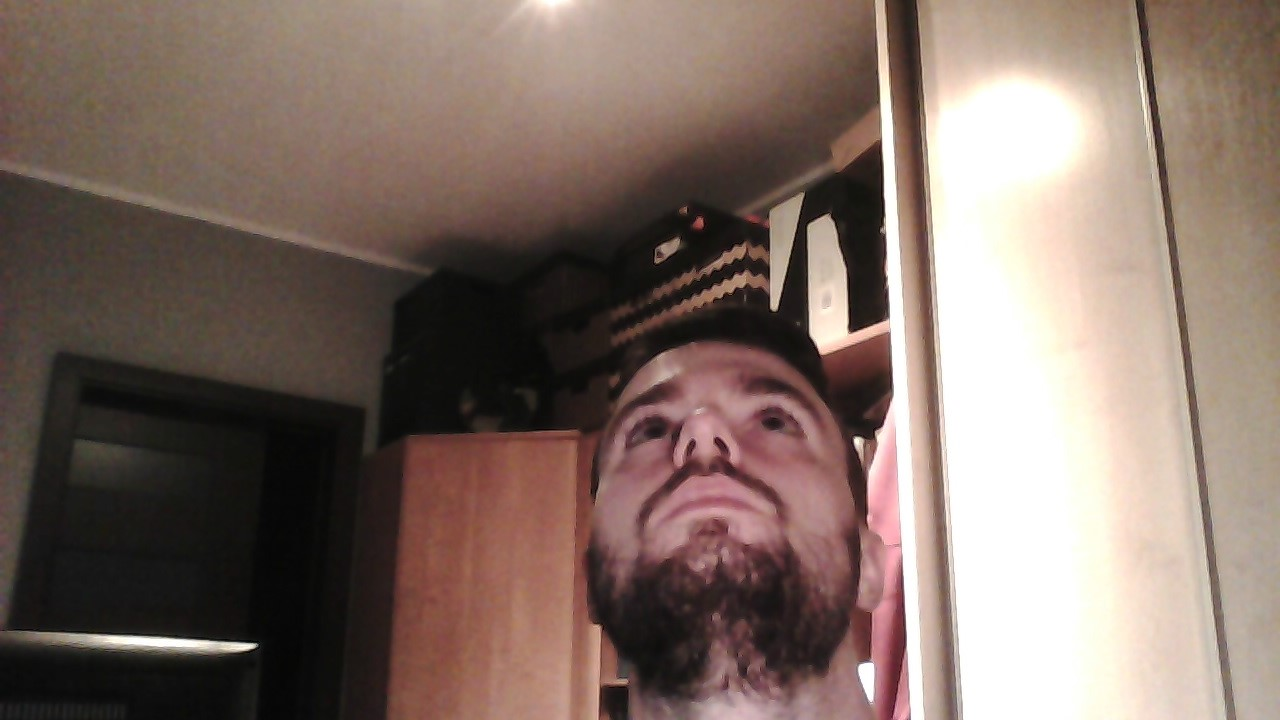
\includegraphics[width=\linewidth, height=20mm]{detekcja/6_input.jpg}
    	\end{minipage}
		& 
		\begin{minipage}{.2\textwidth}
      	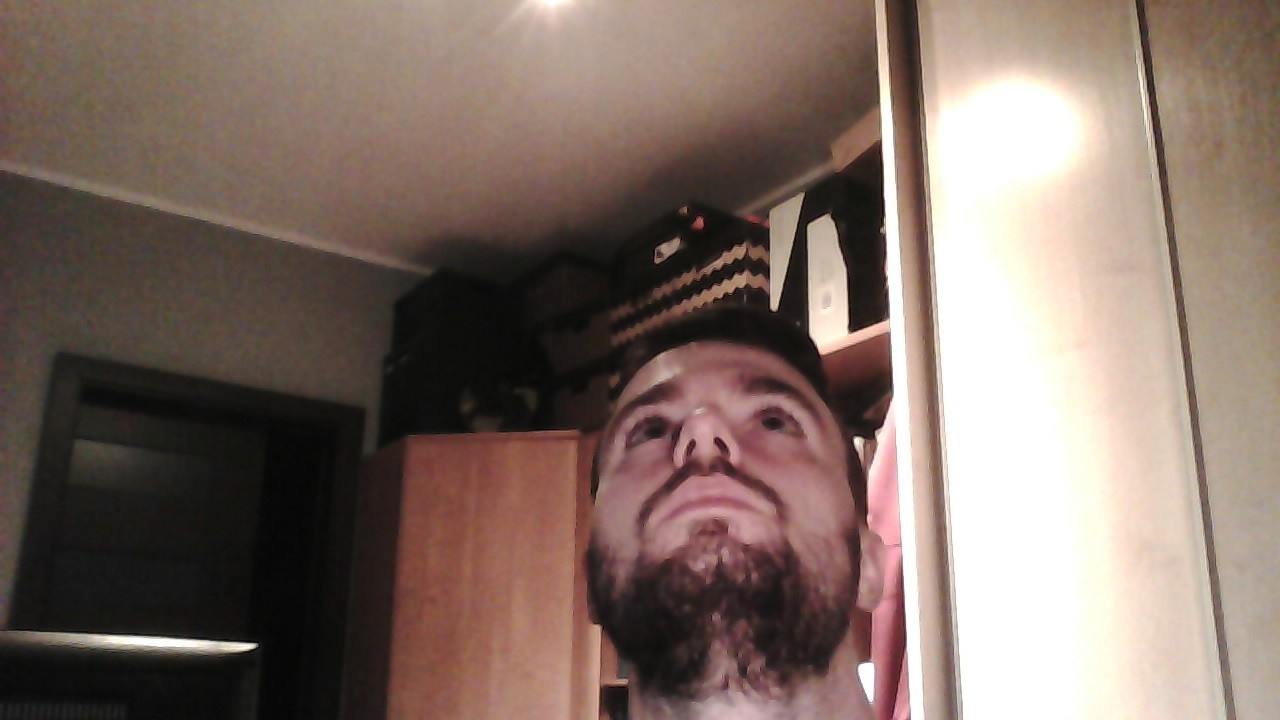
\includegraphics[width=\linewidth, height=20mm]{detekcja/6_haar.jpg}
    	\end{minipage}
		& 
		\begin{minipage}{.2\textwidth}
      	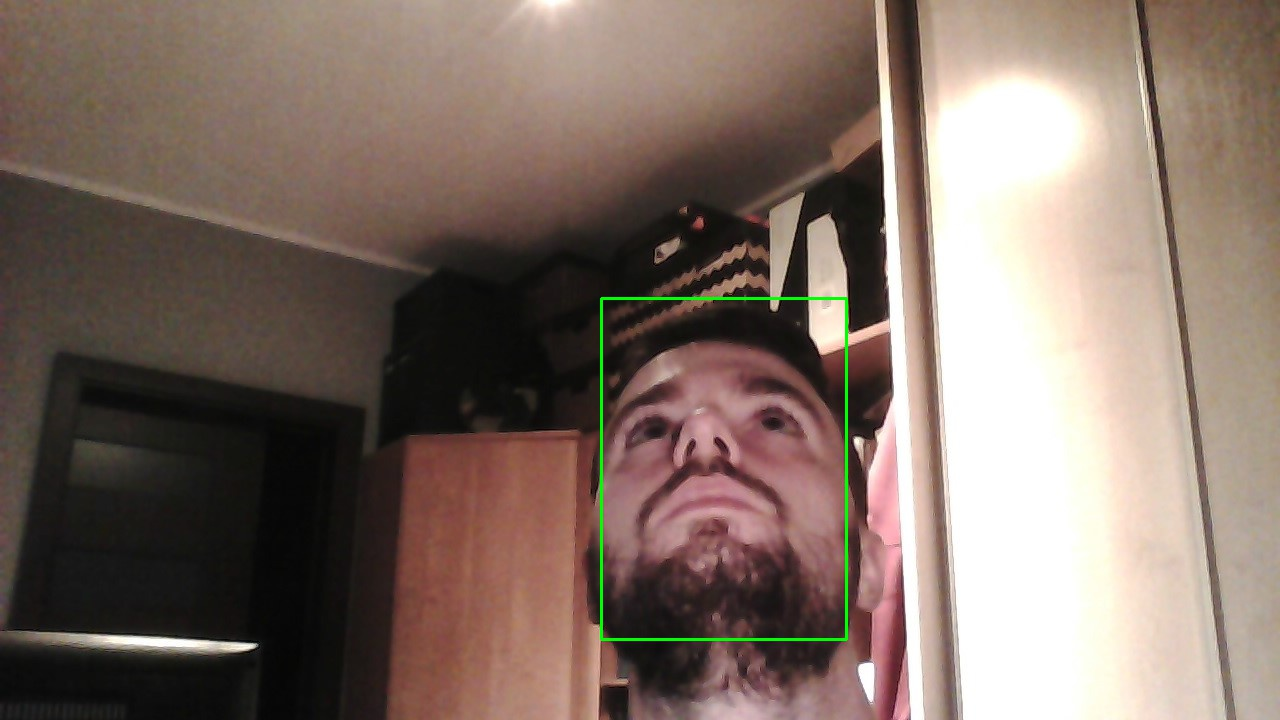
\includegraphics[width=\linewidth, height=20mm]{detekcja/6_dnn.jpg}
    	\end{minipage}
		& 
		\begin{minipage}{.2\textwidth}
      	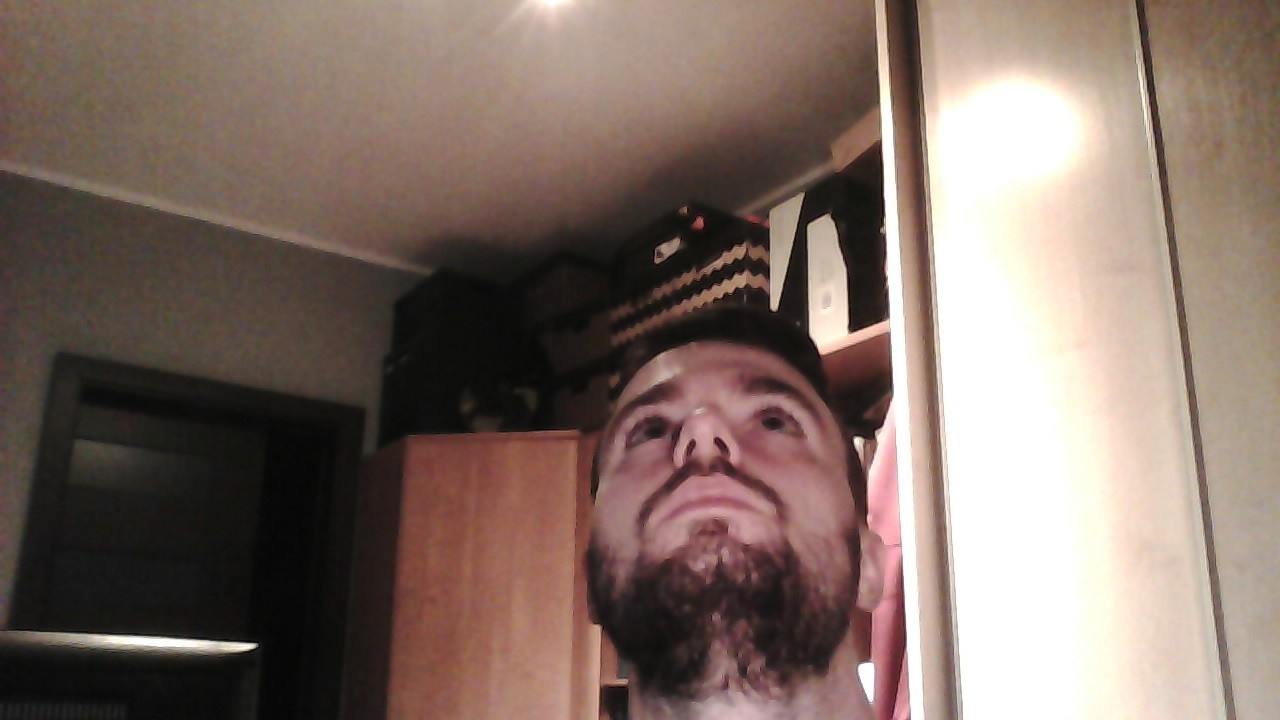
\includegraphics[width=\linewidth, height=20mm]{detekcja/6_azure.jpg}
    	\end{minipage}	
		\\
  		\hline
  		5&  		\begin{minipage}{.2\textwidth}
      	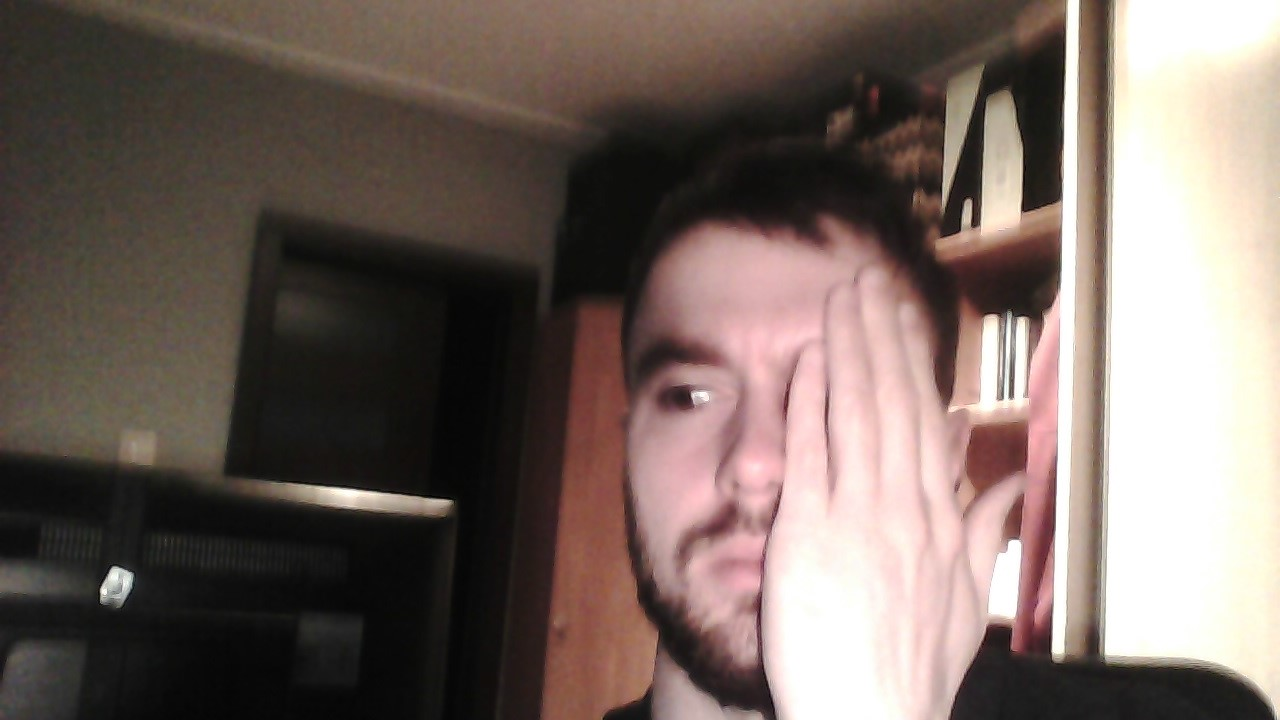
\includegraphics[width=\linewidth, height=20mm]{detekcja/7_input.jpg}
    	\end{minipage}
		& 
		\begin{minipage}{.2\textwidth}
      	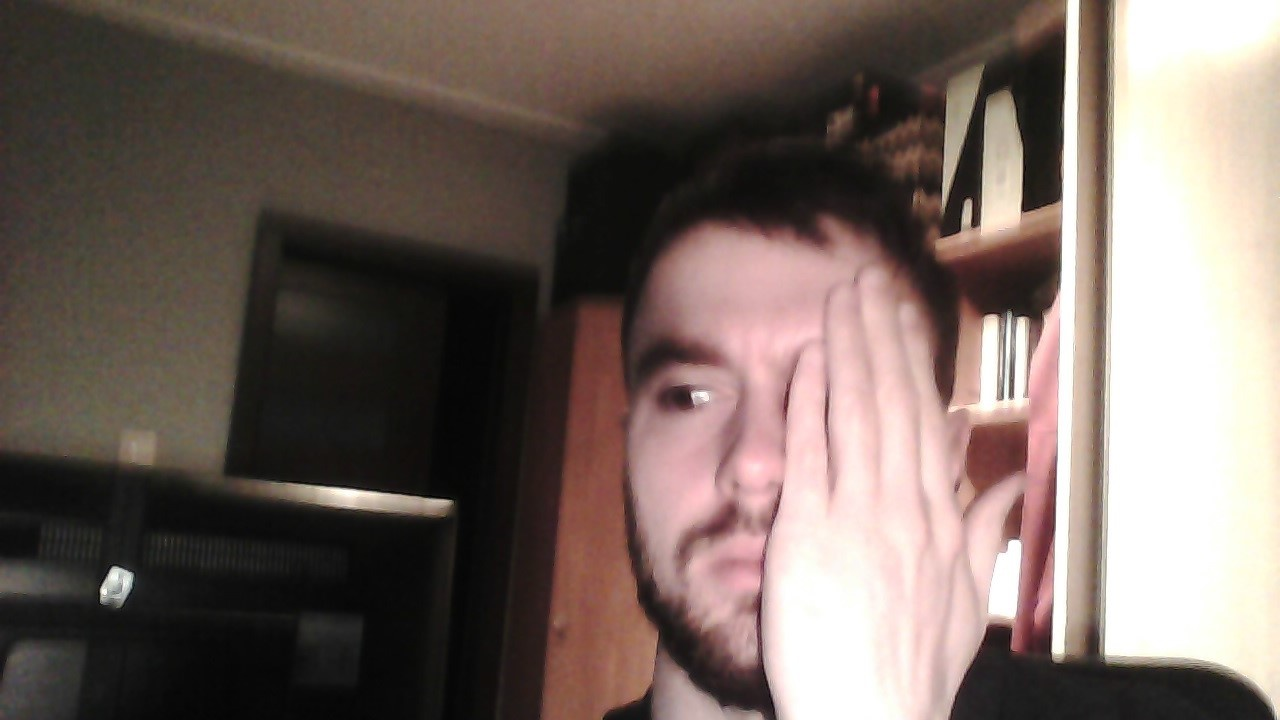
\includegraphics[width=\linewidth, height=20mm]{detekcja/7_haar.jpg}
    	\end{minipage}
		& 
		\begin{minipage}{.2\textwidth}
      	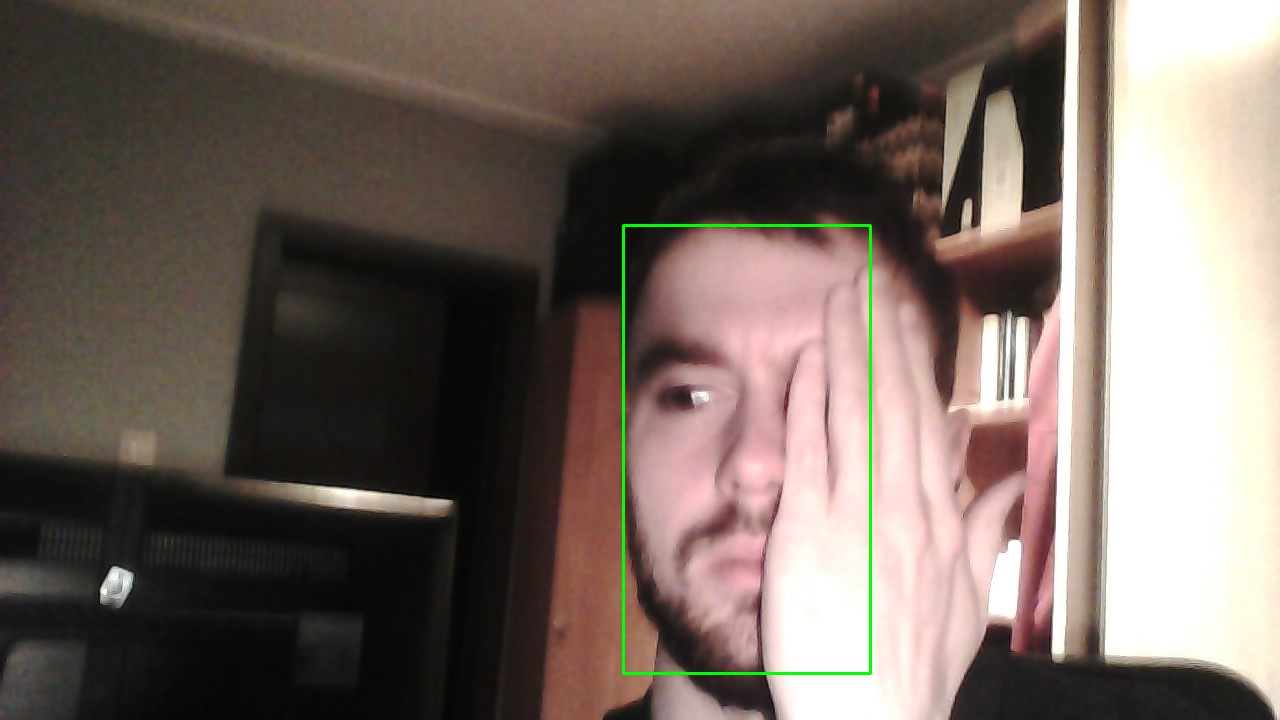
\includegraphics[width=\linewidth, height=20mm]{detekcja/7_dnn.jpg}
    	\end{minipage}
		& 
		\begin{minipage}{.2\textwidth}
      	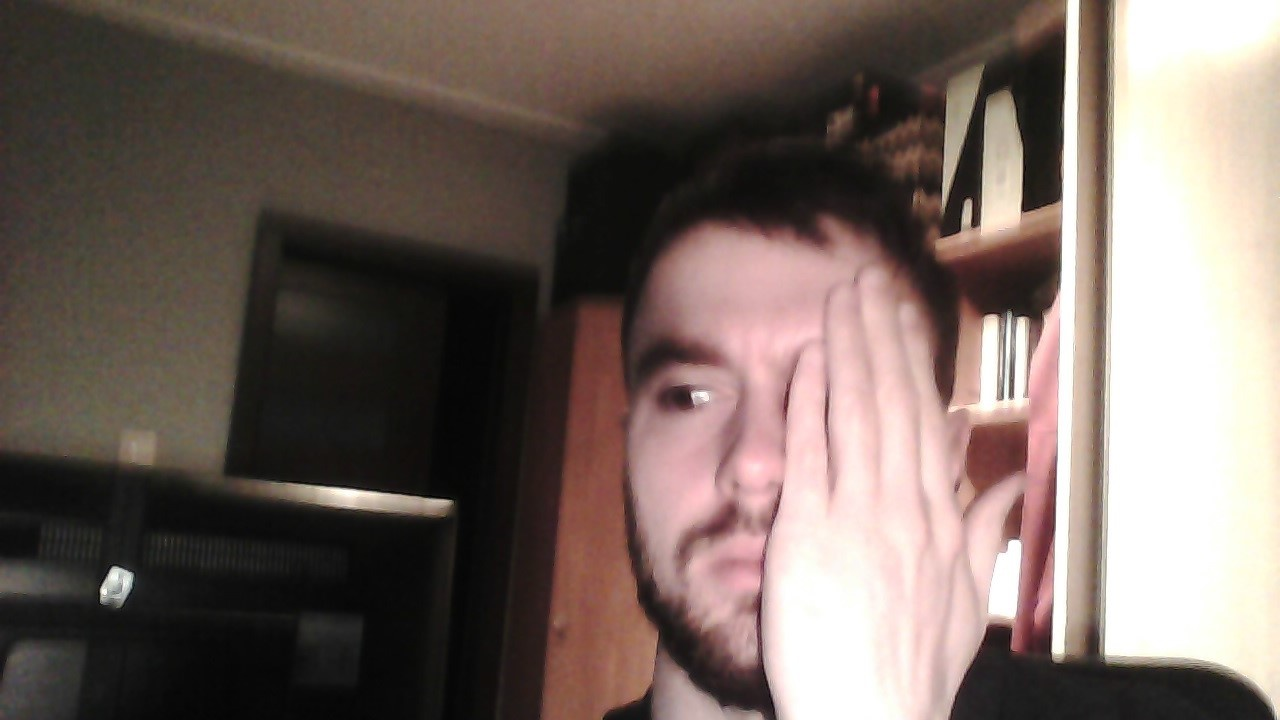
\includegraphics[width=\linewidth, height=20mm]{detekcja/7_azure.jpg}
    	\end{minipage}	
		\\
  		\hline
  		6&  		\begin{minipage}{.2\textwidth}
      	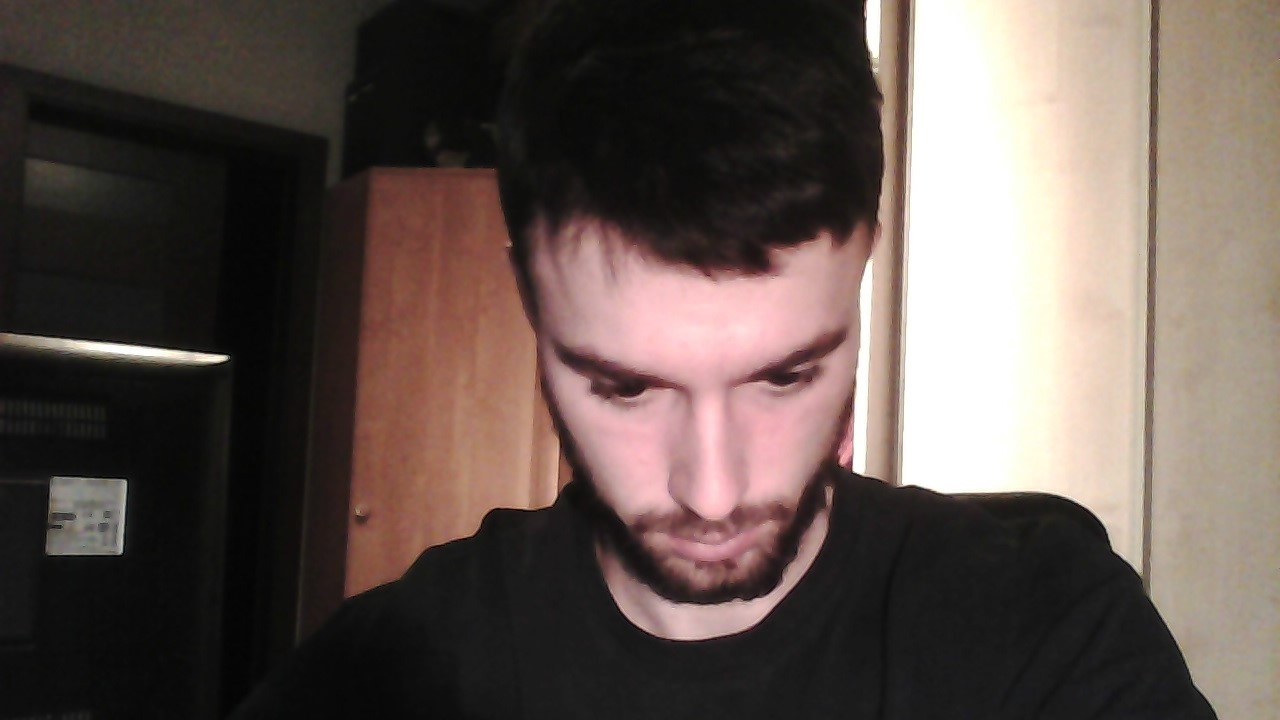
\includegraphics[width=\linewidth, height=20mm]{detekcja/8_input.jpg}
    	\end{minipage}
		& 
		\begin{minipage}{.2\textwidth}
      	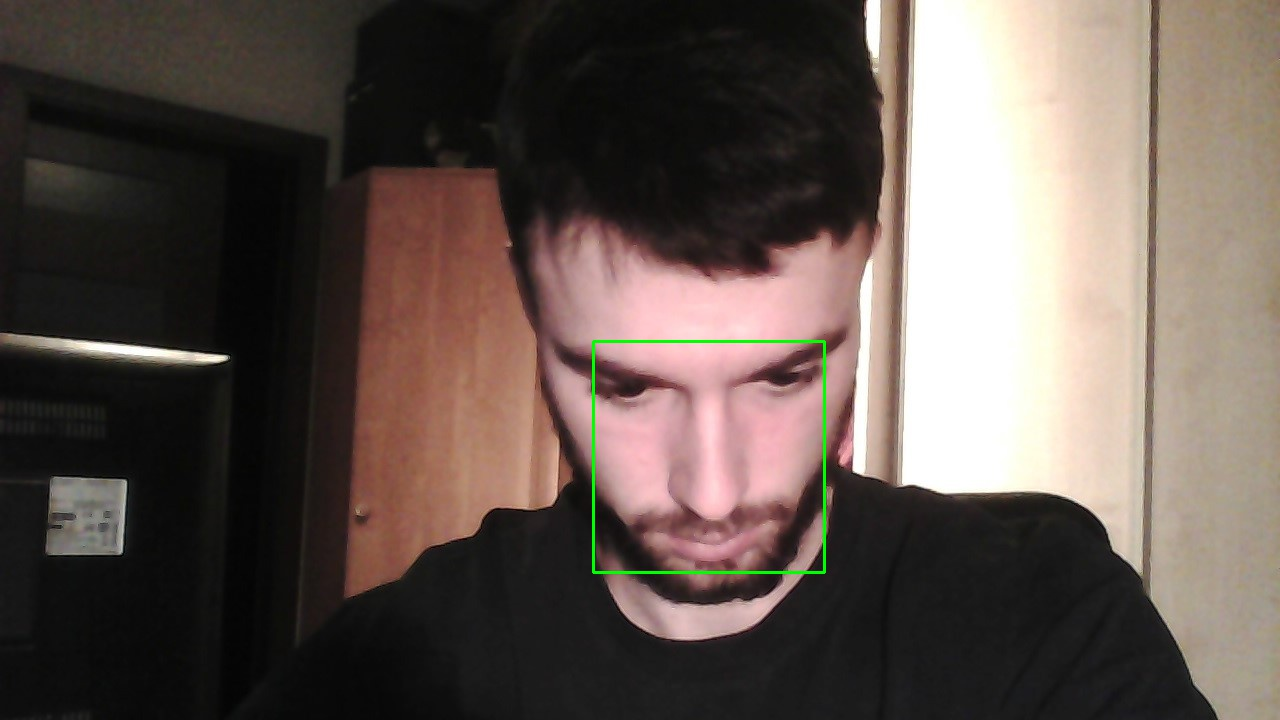
\includegraphics[width=\linewidth, height=20mm]{detekcja/8_haar.jpg}
    	\end{minipage}
		& 
		\begin{minipage}{.2\textwidth}
      	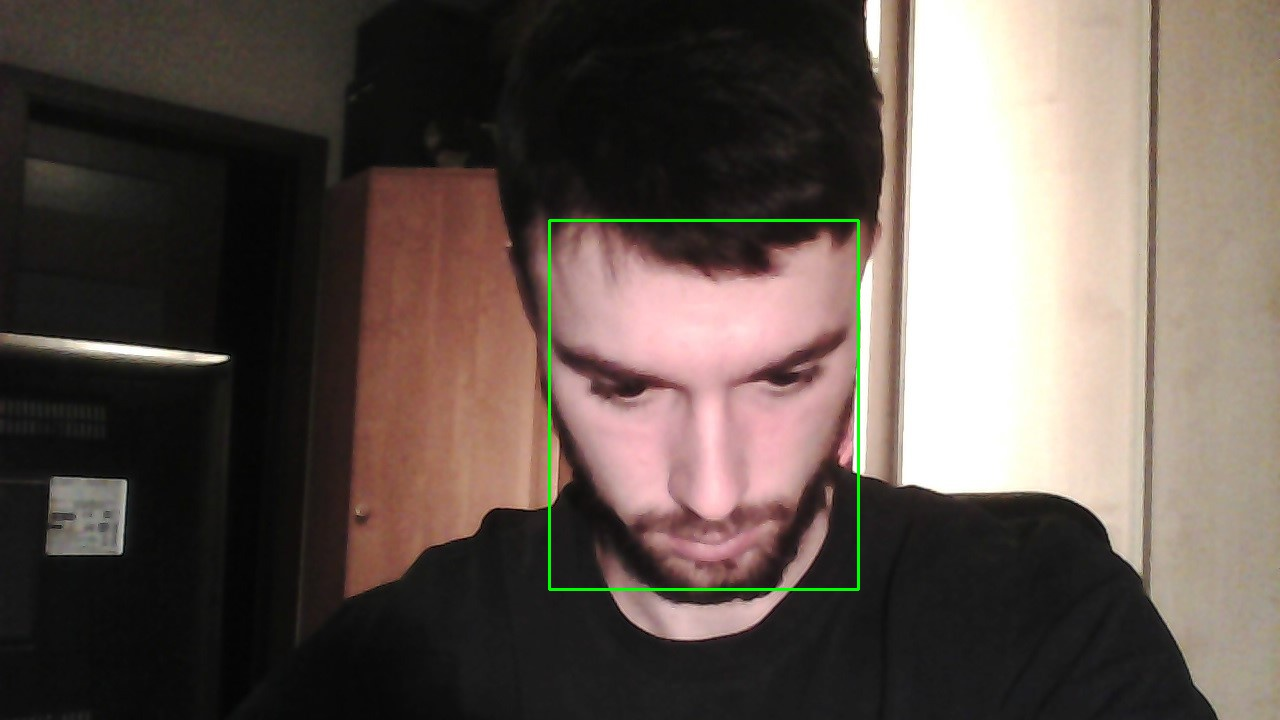
\includegraphics[width=\linewidth, height=20mm]{detekcja/8_dnn.jpg}
    	\end{minipage}
		& 
		\begin{minipage}{.2\textwidth}
      	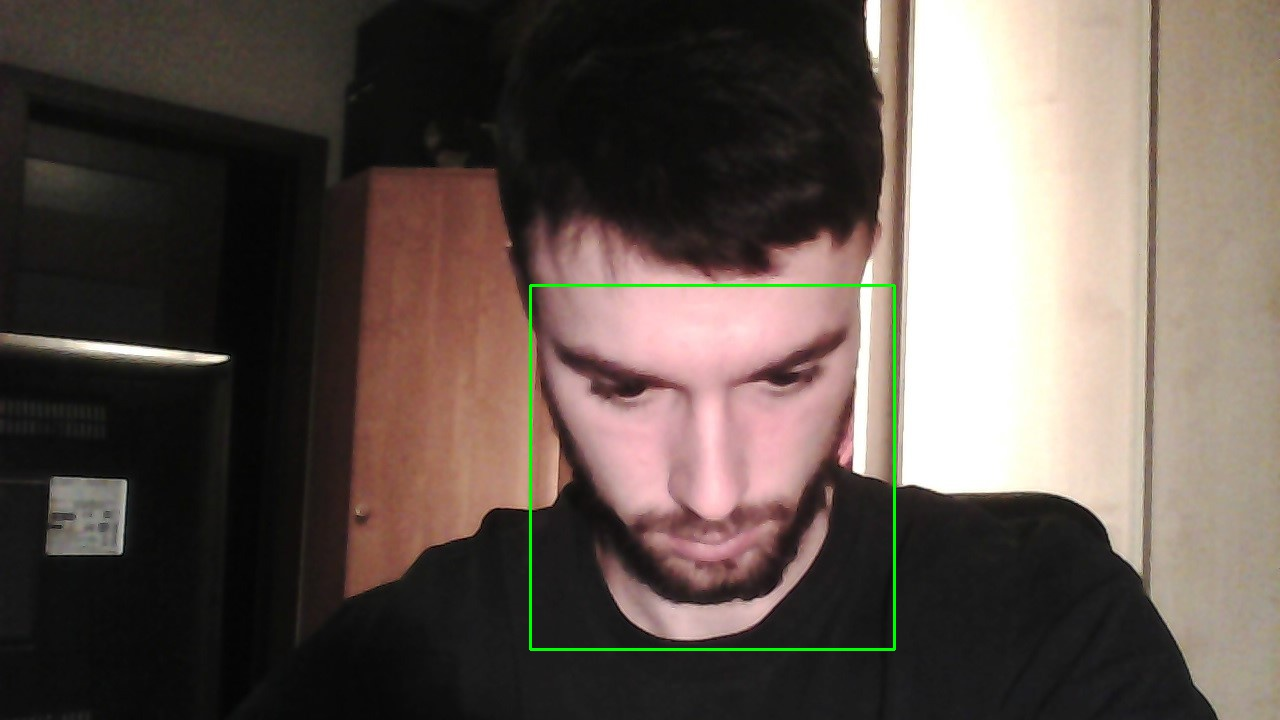
\includegraphics[width=\linewidth, height=20mm]{detekcja/8_azure.jpg}
    	\end{minipage}	
		\\
  		\hline
  		7&  		\begin{minipage}{.2\textwidth}
      	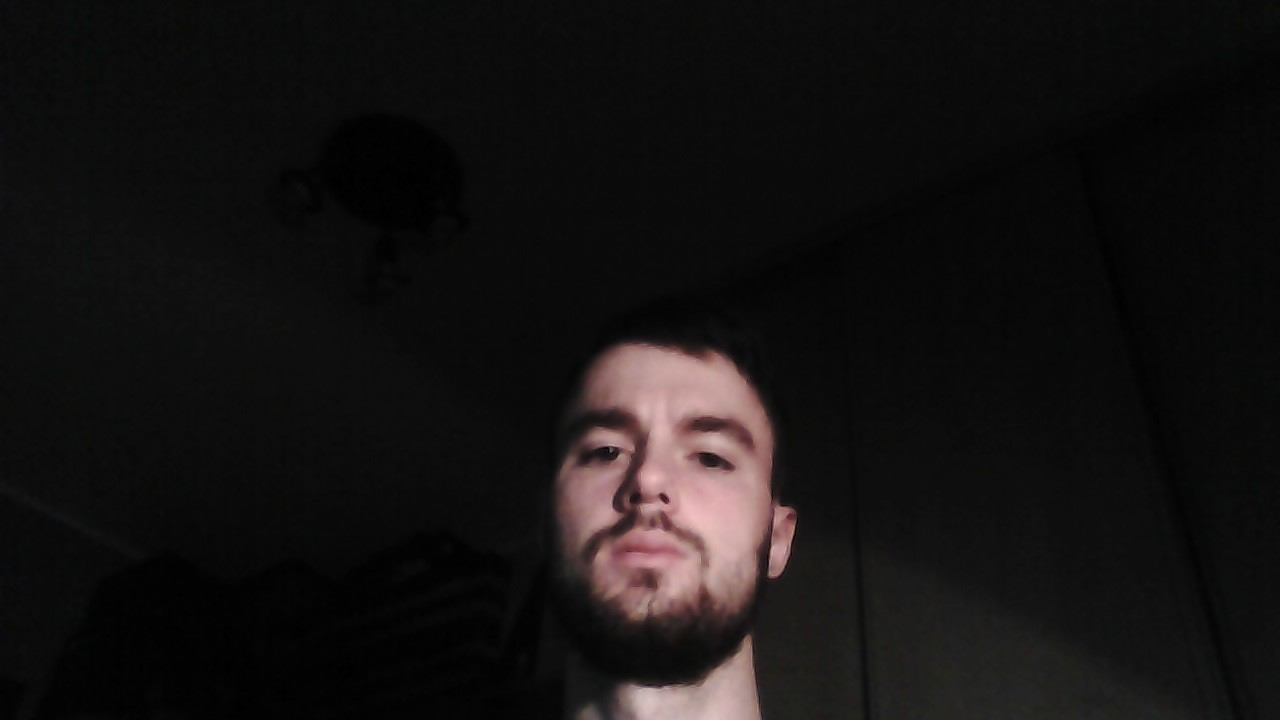
\includegraphics[width=\linewidth, height=20mm]{detekcja/9_input.jpg}
    	\end{minipage}
		& 
		\begin{minipage}{.2\textwidth}
      	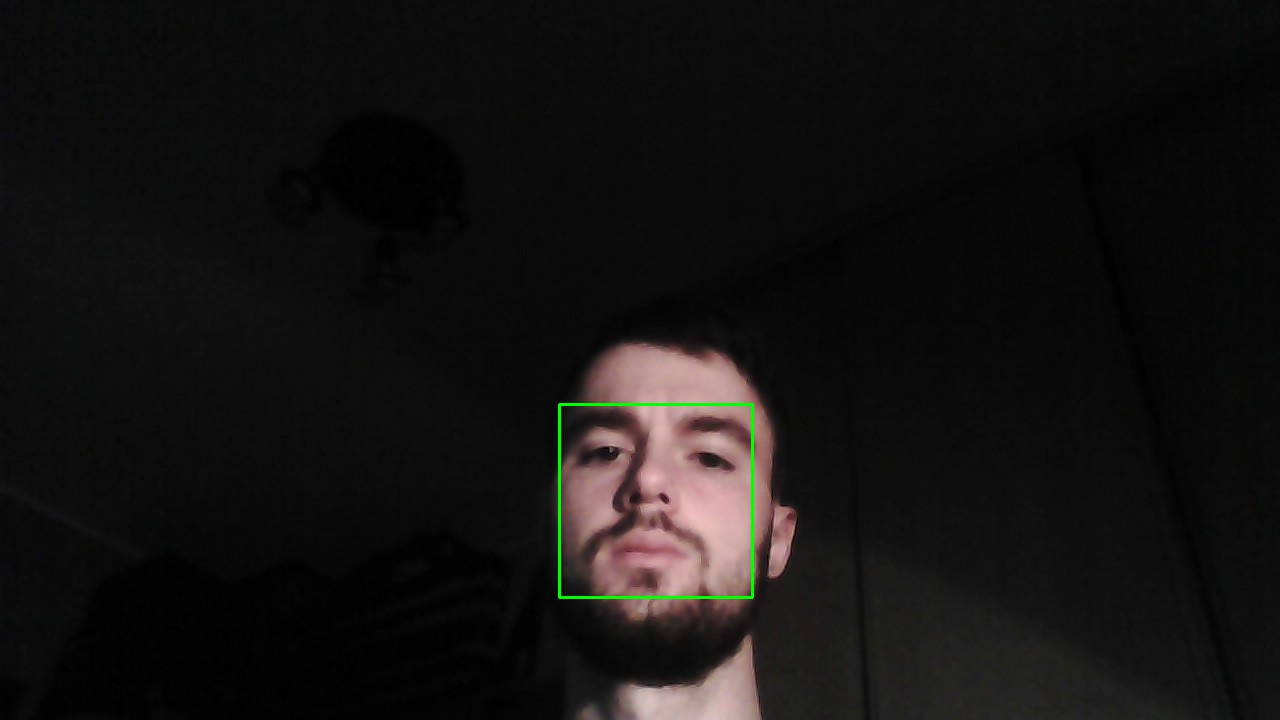
\includegraphics[width=\linewidth, height=20mm]{detekcja/9_haar.jpg}
    	\end{minipage}
		& 
		\begin{minipage}{.2\textwidth}
      	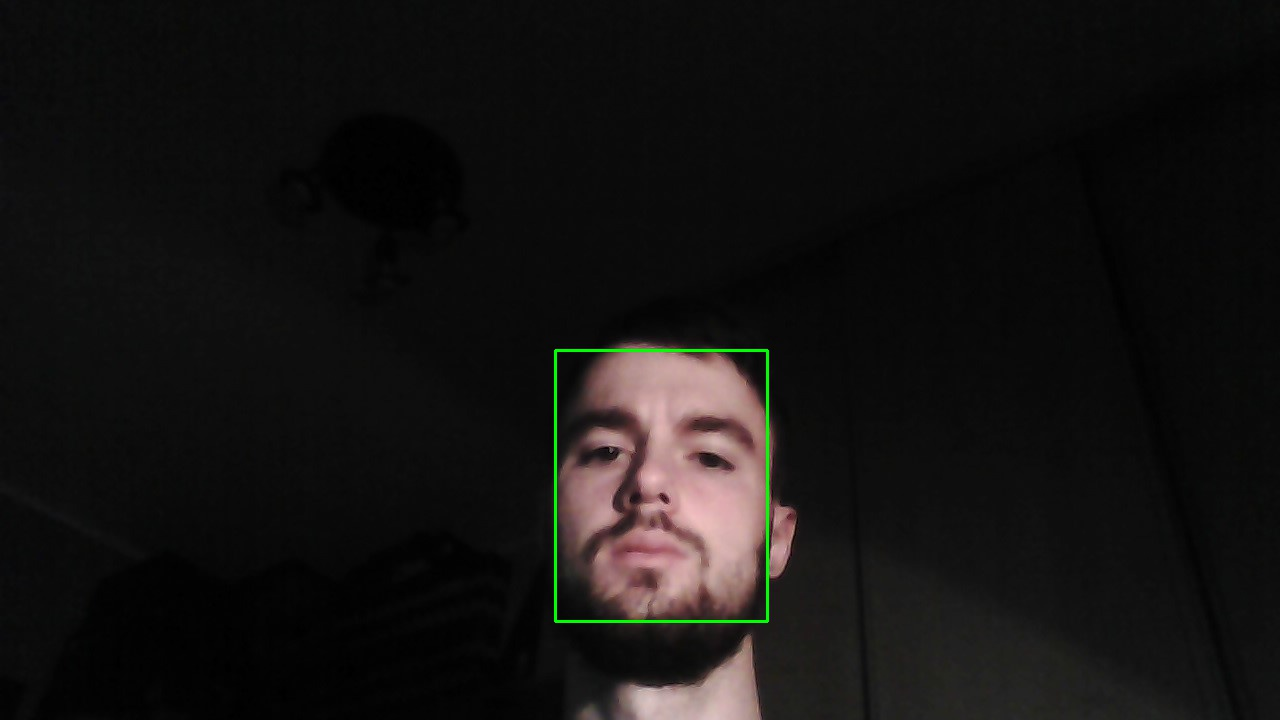
\includegraphics[width=\linewidth, height=20mm]{detekcja/9_dnn.jpg}
    	\end{minipage}
		& 
		\begin{minipage}{.2\textwidth}
      	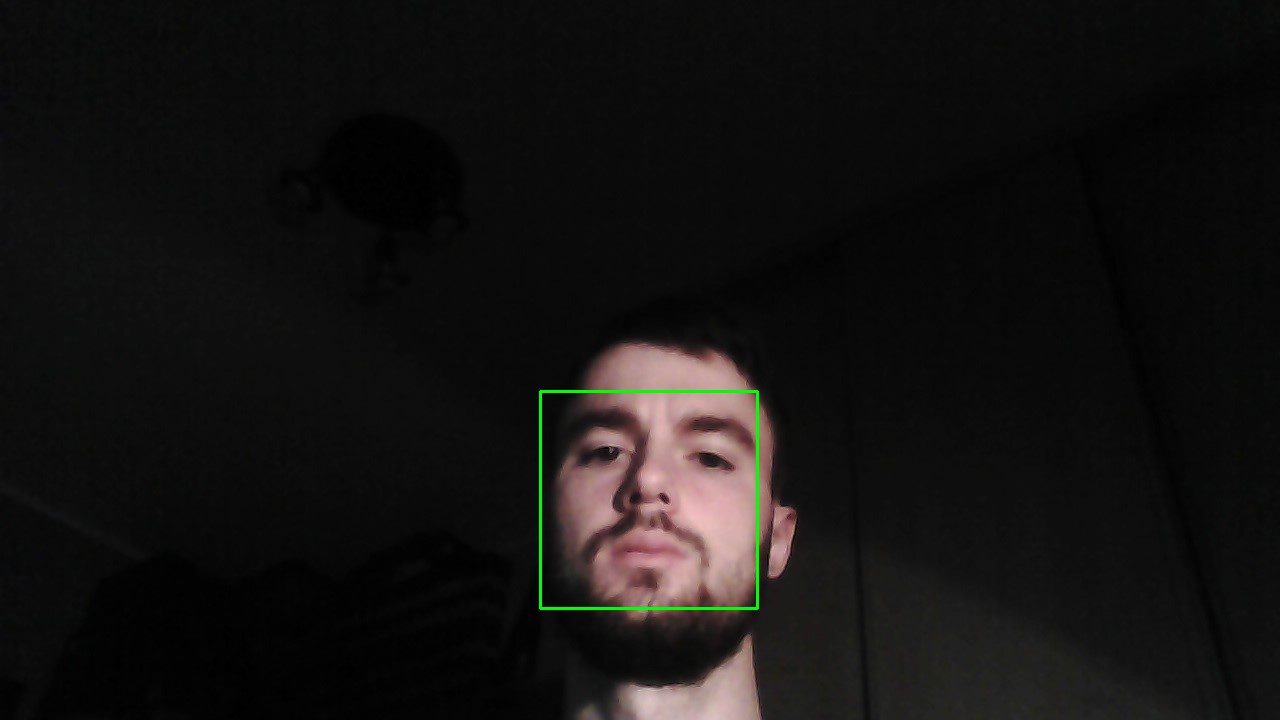
\includegraphics[width=\linewidth, height=20mm]{detekcja/9_azure.jpg}
    	\end{minipage}	
		\\
  		\hline
  		8&  		  		\begin{minipage}{.2\textwidth}
      	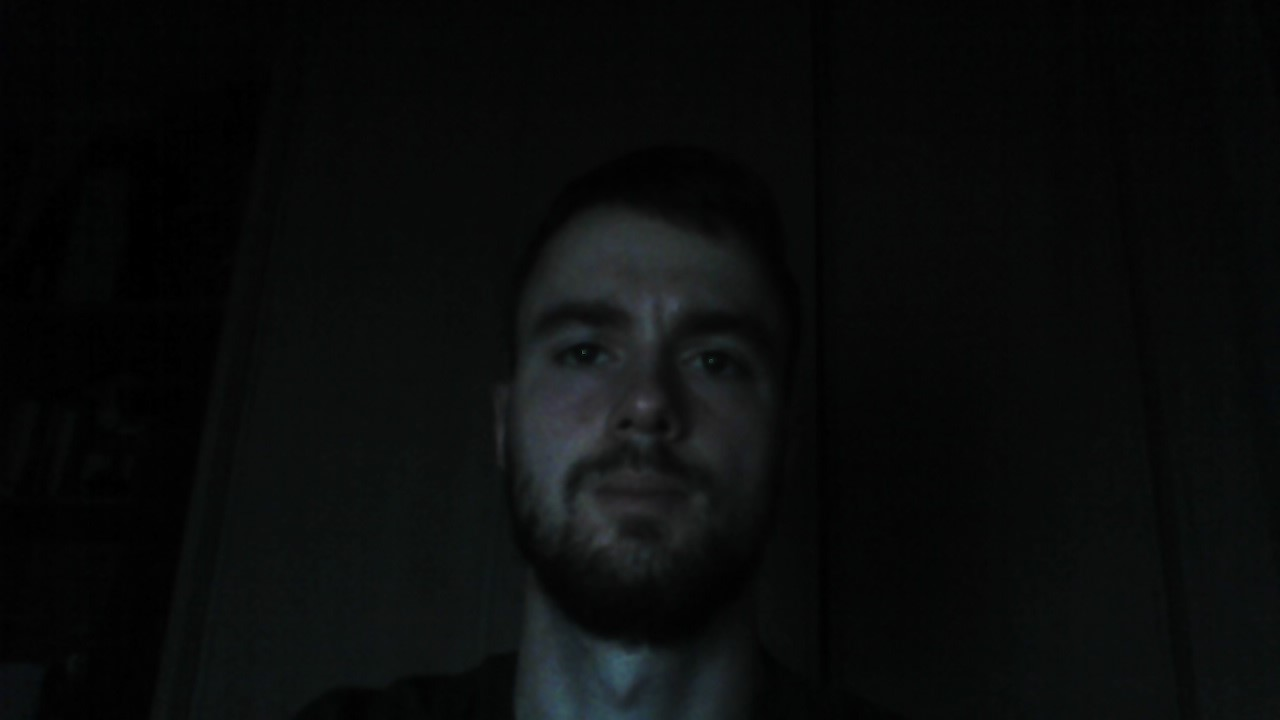
\includegraphics[width=\linewidth, height=20mm]{detekcja/11_input.jpg}
    	\end{minipage}
		& 
		\begin{minipage}{.2\textwidth}
      	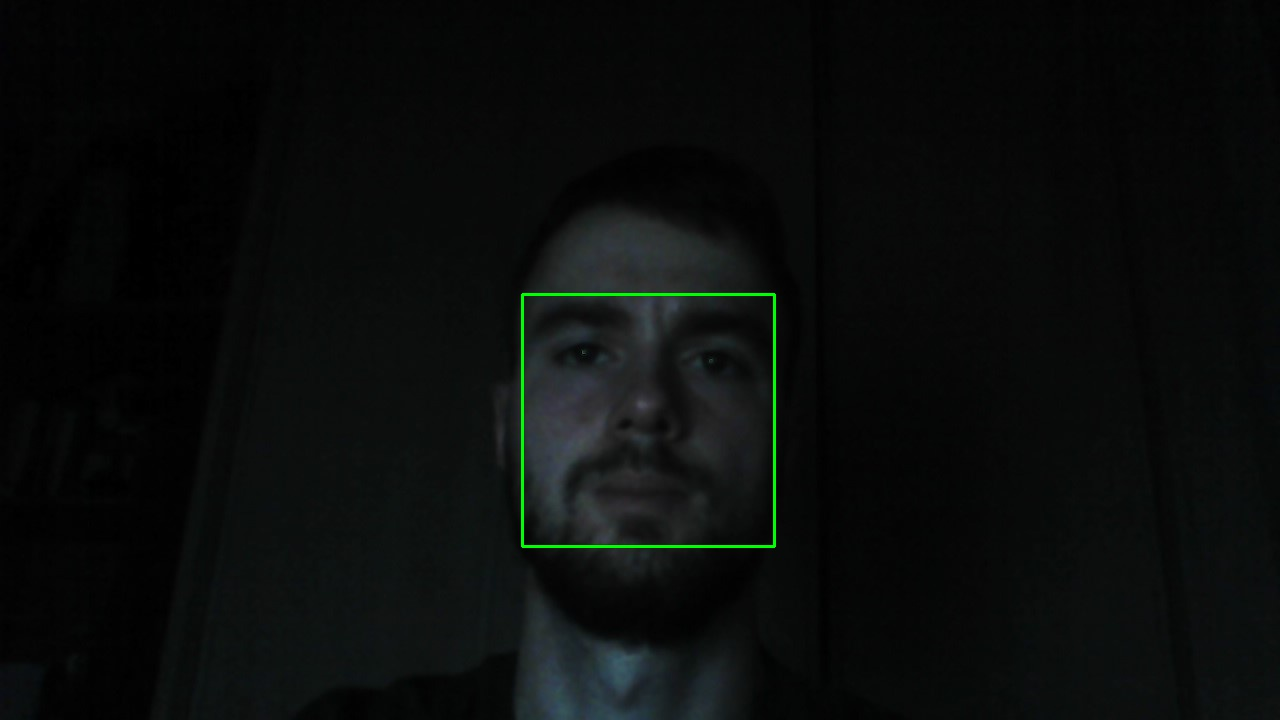
\includegraphics[width=\linewidth, height=20mm]{detekcja/11_haar.jpg}
    	\end{minipage}
		& 
		\begin{minipage}{.2\textwidth}
      	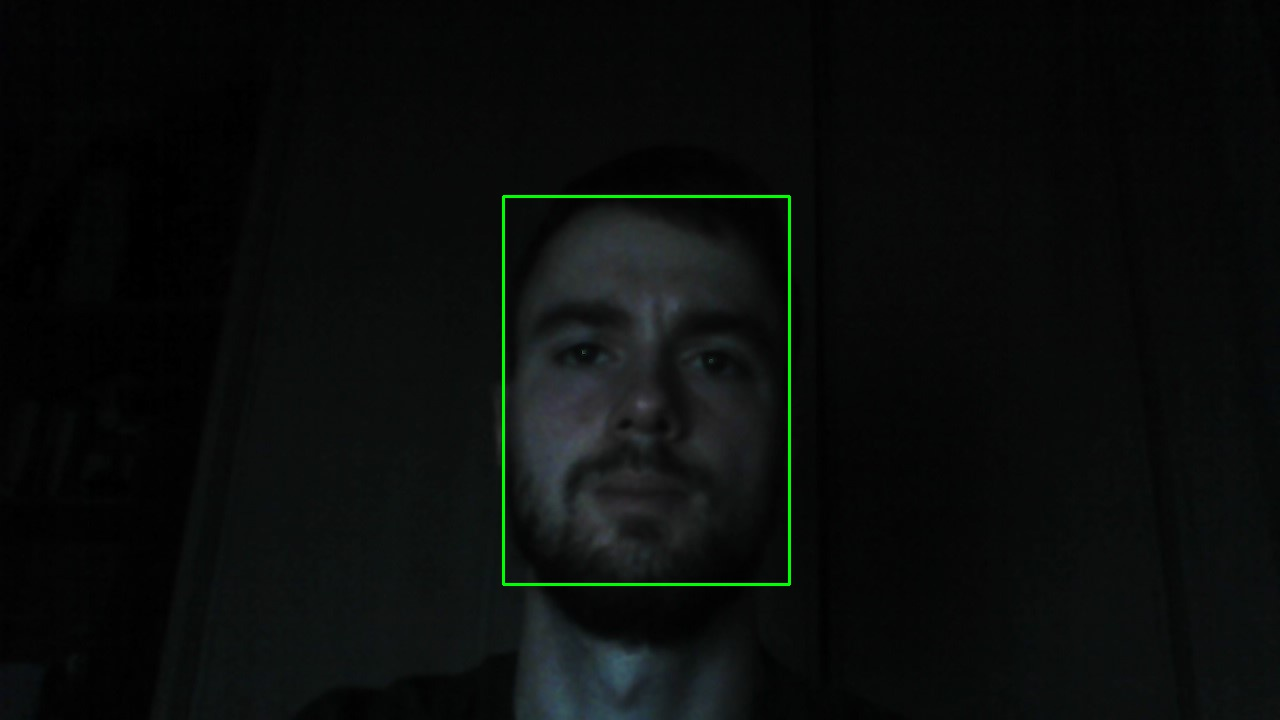
\includegraphics[width=\linewidth, height=20mm]{detekcja/11_dnn.jpg}
    	\end{minipage}
		& 
		\begin{minipage}{.2\textwidth}
      	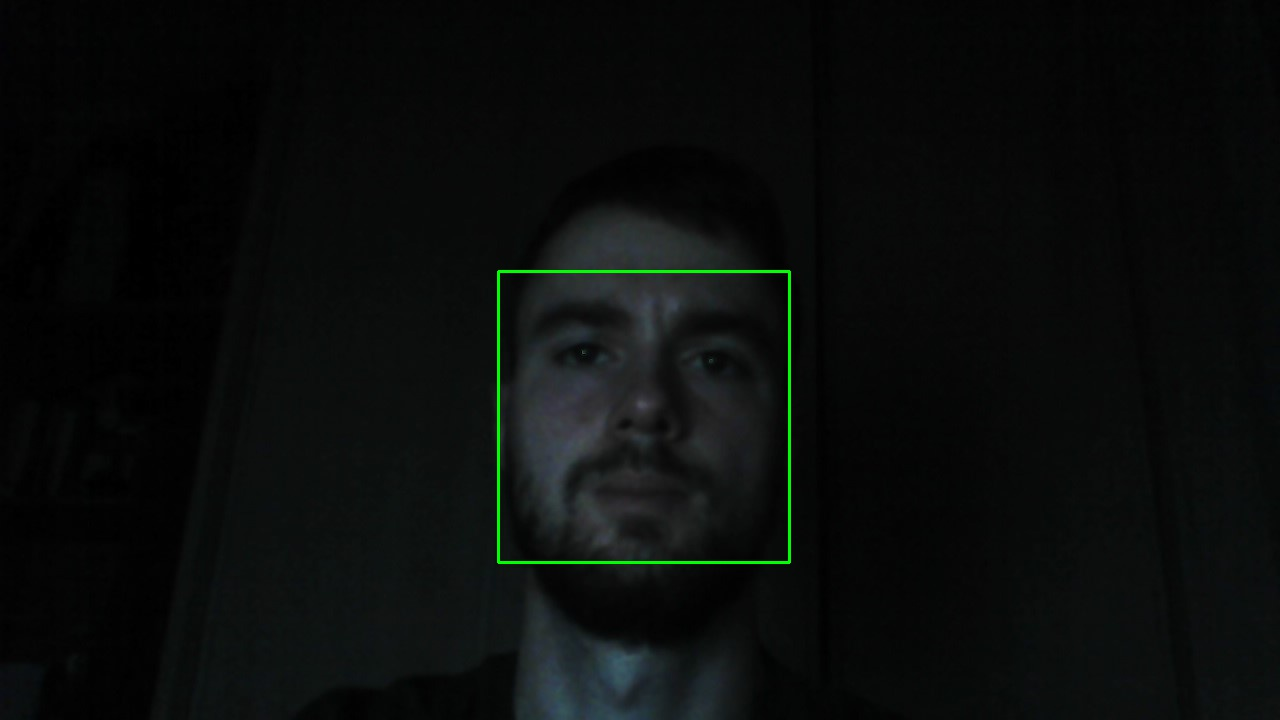
\includegraphics[width=\linewidth, height=20mm]{detekcja/11_azure.jpg}
    	\end{minipage}	
		\\
  		\hline
  		9&  		  		\begin{minipage}{.2\textwidth}
      	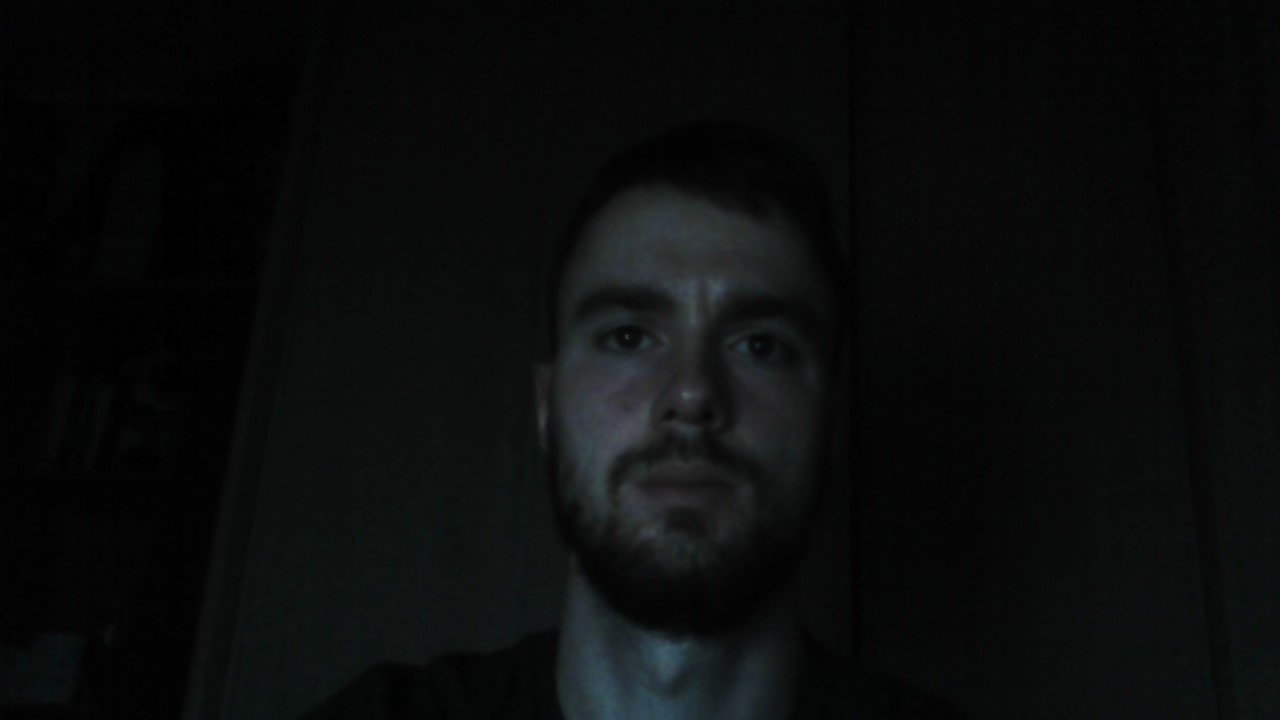
\includegraphics[width=\linewidth, height=20mm]{detekcja/12_input.jpg}
    	\end{minipage}
		& 
		\begin{minipage}{.2\textwidth}
      	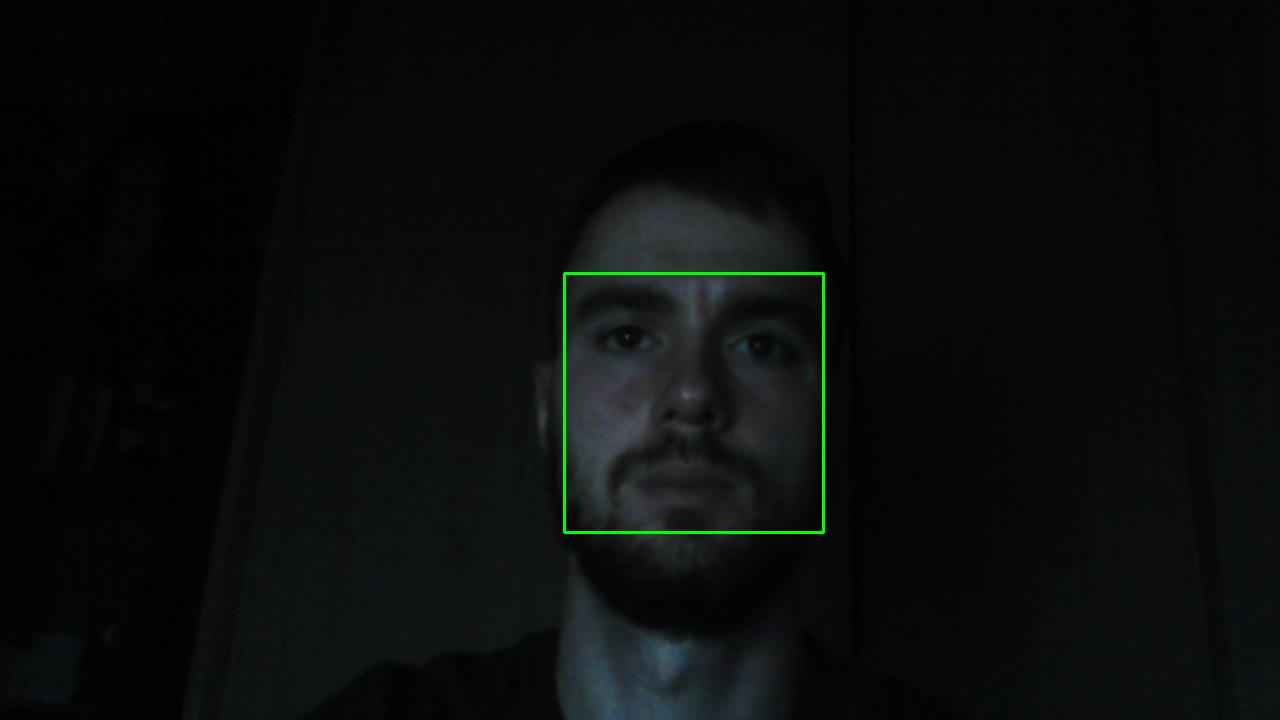
\includegraphics[width=\linewidth, height=20mm]{detekcja/12_haar.jpg}
    	\end{minipage}
		& 
		\begin{minipage}{.2\textwidth}
      	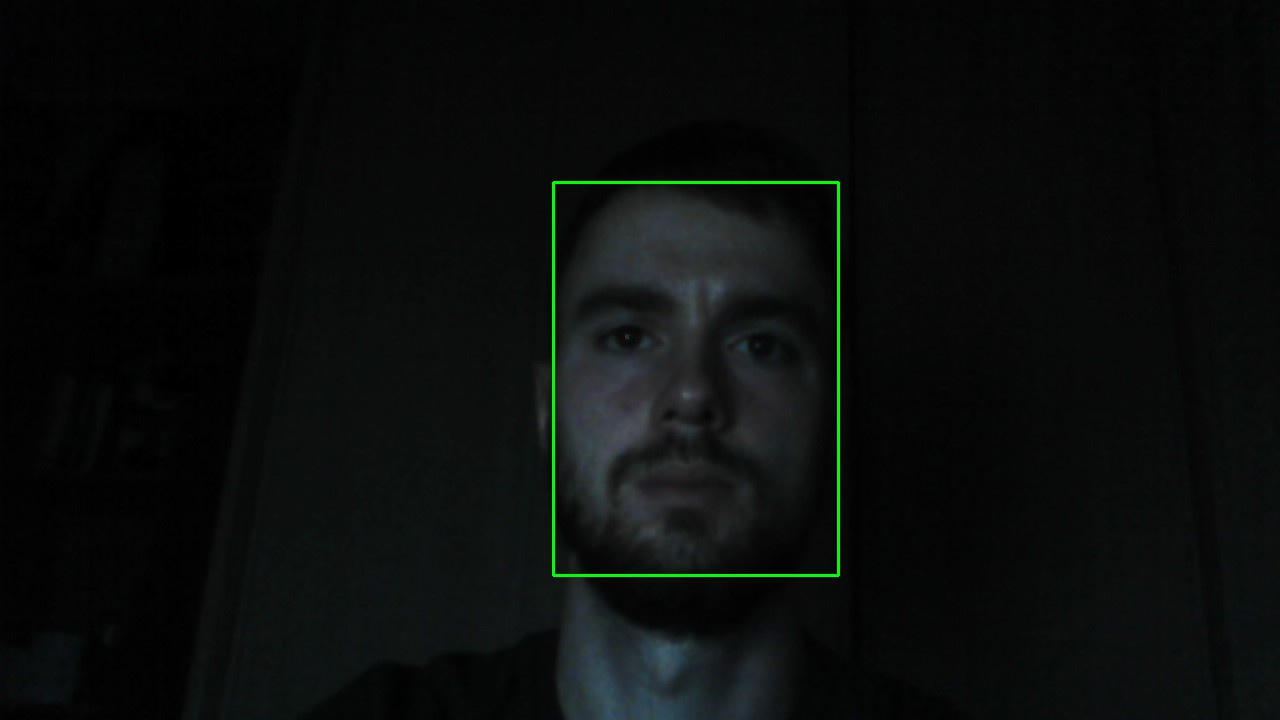
\includegraphics[width=\linewidth, height=20mm]{detekcja/12_dnn.jpg}
    	\end{minipage}
		& 
		\begin{minipage}{.2\textwidth}
      	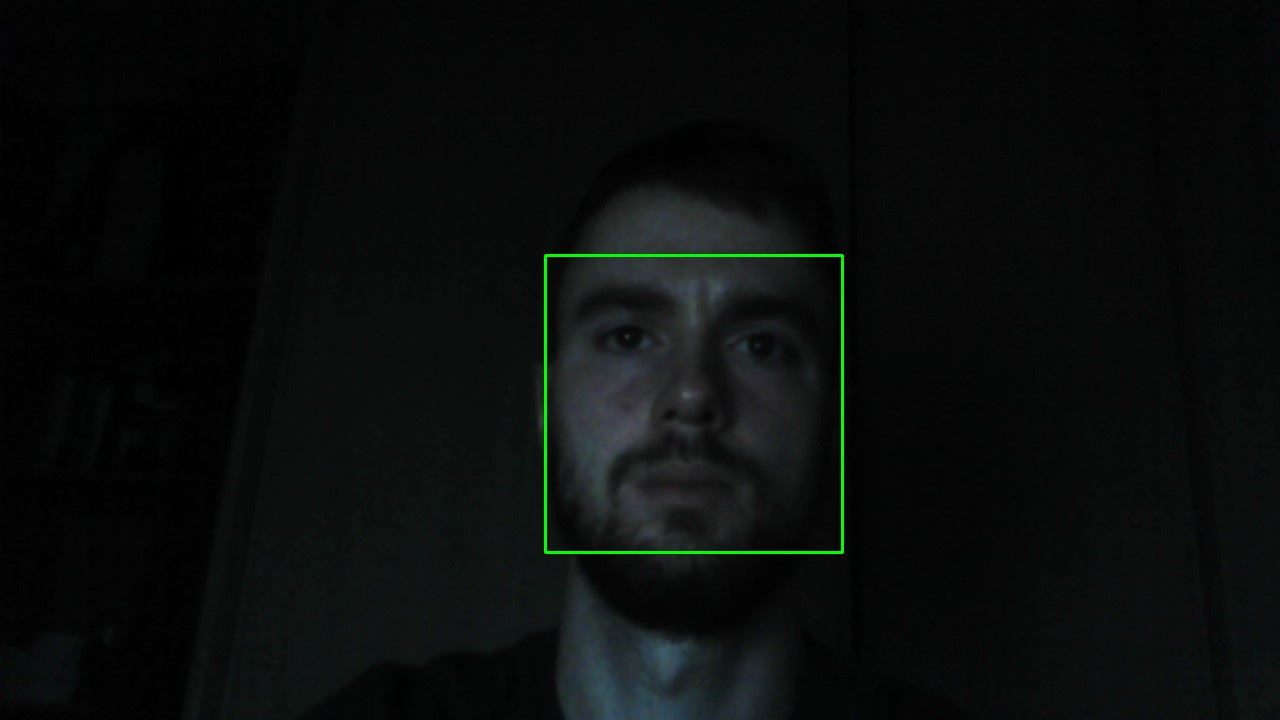
\includegraphics[width=\linewidth, height=20mm]{detekcja/12_azure.jpg}
    	\end{minipage}	
    	\\
  		\hline 
\caption{Porównanie działania detektorów w wybranych warunkach}
\label{tab:porownanie_detektorow}
\end{longtable}
Pierwszą różnicą, którą można zaobserwować w sposobie działania detektorów jest rozmiar obszaru twarzy oznaczany przez algorytmy. Najmniejszym z nich jest twarz wykrywana metodą Haara, oznaczany obszar zaczyna się na wysokości brwi i kończy niewiele poniżej ust. W przypadku detekcji twarzy z wykorzystaniem głębokiej sieci neuronowej prostokąt obejmuje także całe czoło oraz podbródek przedstawionej osoby. Rozmiar obszaru uzyskanego przez ACS(Azure Cognitive Services) mieści się pomiędzy metodą Haara a DNN(Deep Neural Network), obejmuję częściowo czoło i podbródek.

Każda z metod dobrze poradziła sobie w przypadku centralnego zdjęcia twarzy przy dobrym jak i słabym oświetleniu. Najskuteczniejszą z metod okazała się metoda DNN, która wykryła twarz na każdym z dziewięciu zdjęć. Metoda wykorzystująca platformę Azure okazała się nieskuteczna w przypadku zdjęcia przedstawiającego częściowo zakrytą twarz oraz z odchyloną głową. 

Najwrażliwszym na jakoś zdjęcia okazała się metoda Haara, która nie była w stanie sobie poradzić choćby z najmniejszymi zmianami w układzie twarzy na zdjęciu. Używając tego detektora nie udało się wykryć twarzy na obrazach, które nie sprawiły problemu pozostałym metodą. Między innymi nie wykryto twarzy na obrazie przedstawiającym profil oraz głowę przechyloną na bok.

Zbadano, że wysoka skuteczność detekcji twarzy metodą DNN wiąże się z większą ilością fałszywych detekcji w porównaniu z pozostałymi metodami. Z tego powodu wyniki uzyskane tą metodą należy filtrować,a jest to możliwe poprzez ustawienie pewności powyżej, której algorytm ma zwracać odpowiedzi.

Średnie czasy odpowiedzi detektorów przedstawiono w tabeli \ref{tab:systemy}. W najkrótszym czasie uzyskano odpowiedź od sieci neuronowej, a najwolniejsza zgodnie z oczekiwania była metoda wykorzystująca ACS. Znacznie dłuższy czas trwania wynika z konieczności skontaktowania się z serwerem z innego kraju.

\begin{table}[H]\label{tab:systemy}
	\centering
	\caption{Średni czas przetwarzania zadania detekcji twarzy}
	\scalebox{1.0}{
	\begin{tabular}{|c|c|c|c|}
  		\hline 
  		 & \bfseries Haar & \bfseries Dnn & \bfseries ACS\\
  		\hline
  		\bfseries Średni czas odpowiedzi [s]& 0,023127109 &0,018201053 &0,465438843 \\
  		\hline
  	\end{tabular}
  	}
\end{table}

W celu potwierdzenia uzyskanych wniosków przeprowadzono końcowy test polegający na uruchomieniu każdego z detektorów na bazie profili składającej się z 2000 zdjęć. Wyniki przedstawiono na rysunku \ref{fig:porownanie_detektorow}. Detektor oparty o głęboką siec neuronową wykrył twarz na 94,6\% zdjęć, Azure 90,1\%, a Haar 88,7\%. Wyniki potwierdziły, że sieć neuronowa, w tym przypadku daje najlepsze rezultaty, korzystniejsze o nawet 6\% od pozostałych metod.

\begin{figure}[H]
	\centering
	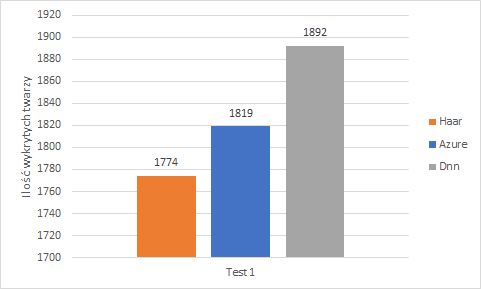
\includegraphics[scale=1.0]{porownanie_detektorow.png}
	\caption{Porównanie działania detektorów na bazie 2000 zdjęć}
	\label{fig:porownanie_detektorow}
\end{figure}

\section{Dane treningowe}
Za dane wejściowe do procesu trenowania sieci neuronowych wybrano \fnurl{Glasgow Unfamiliar Face Database (GUFD)}{http://www.facevar.com/glasgow-unfamiliar-face-database}, która dostępna jest za darmo i można jej używać na potrzeby badań uczelnianych oraz publikacji. Jedynym warunkiem użycia jest zacytowanie jednej z publikacji właściciela bazy.

Baza zawiera 303 tożsamości. Na każdą z tożsamości składa się 20 zdjęć jednej osoby wykonanych w różnych warunkach np. różniące się kąty ujęcia, wyrazy twarzy oraz z dodatkowymi akcesoriami(okulary, kaptur, czapka). 

Do materiałów uczących dodatkowo dodano profil autora tej pracy magisterskiej.

\section{Trenowanie sieci neuronowych}
Podczas badania sieci neuronowych postanowiono sprawdzić kilka podstawowych czynników, na które składa się wpływ ilości wybranych tożsamości oraz wpływ ilości zdjęć przydzielonych tożsamości na:
\begin{itemize}
\item czas potrzebny na preprocessing danych uczących,
\item czas trwania trenowania modelu,
\item rozmiar pliku zawierającego model (jeśli istnieje).
\end{itemize}
W rozdziale \ref{b:rozpoznawanie} omówiono wpływ wyżej wymienionych parametrów na czas oraz pewność identyfikowania tożsamości.

\subsection{Wpływ wybranych parametrów na przygotowanie danych uczących}
Zgodnie z oczekiwaniami, preprocessing danych wymagany przed trenowaniem identyfikatorów powiązanych z biblioteką OpenCv jest znacznie szybszy od Azure. Największą wadą wynikającą z chmurowości  ACS(Azure Cognitive Services) jest konieczność wykonania tysięcy zapytań, w tym większość z nich odpowiadających za przekazanie zdjęć do chmury. Prędkość dodawania danych jest ograniczana przez jakość połączenia z serwerem. Na przygotowanie 19 zdjęć dla 100 profili, system potrzebował około 15 minut, które może się wydawać astronomiczne w porównaniu z 24 sekundami potrzebnymi na przygotowanie danych dla metod trenowanych lokalnie.

Na rysunku \ref{fig:czas_p_profile} można zaobserwować że czas potrzebny na przygotowanie danych w przypadku OpenCv rósł liniowo. Podobny efekt był oczekiwany dla ACS. Brak liniowości może wynikać z różnych rozmiarów plików oraz chwilowej lepszej/gorszej jakości połączenia z serwerem.
\begin{figure}[H]
	\centering
	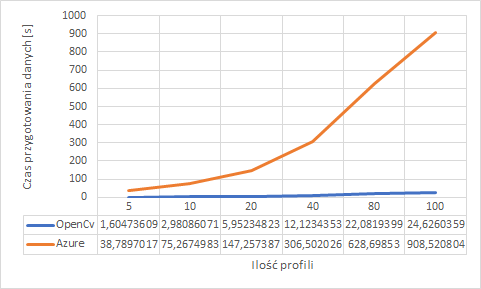
\includegraphics[scale=1.0]{czas_przygotowania_a_ilosc_profili.png}
	\caption{Wpływ ilości profili użytych podczas treningu na czas przygotowania danych uczących}
	\label{fig:czas_p_profile}
\end{figure}
Wyniki uzyskane podczas drugiego testu, które przedstawiono na grafie \ref{fig:czas_p_zdjecia} potwierdzają tezę o niestabilności połączenia z serwisem chmurowym. Dla tego testu udało się uzyskać zależność ilości zdjęć od czasu zbliżoną do liniowej.
\begin{figure}[H]
	\centering
	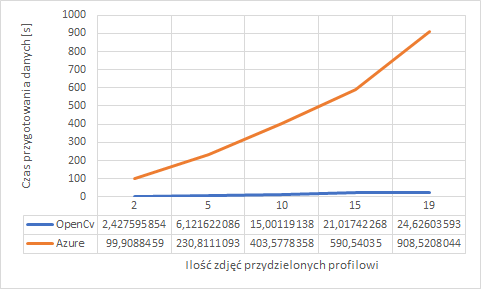
\includegraphics[scale=1.0]{czas_przygotowania_a_ilosc_zdjec.png}
	\caption{Wpływ ilości zdjęć przydzielonych profilowi na czas przygotowania danych uczących}
	\label{fig:czas_p_zdjecia}
\end{figure}

\subsection{Wpływ wybranych parametrów na czas trwania treningu}
Kolejnym interesującym testem, który przeprowadzona było zbadanie wpływu ilości użytych profili oraz ilości zdjęć przypisanych profilowi na czas trwania nauki. Zgodnie z oczekiwaniami wraz z przyrostem danych zwiększał się czas wymagany na wytrenowanie sieci. Wyniki przedstawiono na rysunku \ref{fig:czas_t_profile}. Wyjątkiem pozostało rozwiązanie chmurowe Azure, które niezależnie od ilości danych zawsze trwało sekundę (najmniejsza jednostka czasu, którą można uzyskać od usługi). Podobnym zachowaniem wykazał się algorytm LBPH (\ref{lbph}), w przypadku którego czas treningu wydłuż się od 0,7s do maksymalnie 12s. W przypadku pozostałych metod czas treningu wzrósł z początkowej wartości maksymalnie kilku sekund do nawet kilku minut
\begin{figure}[H]
	\centering
	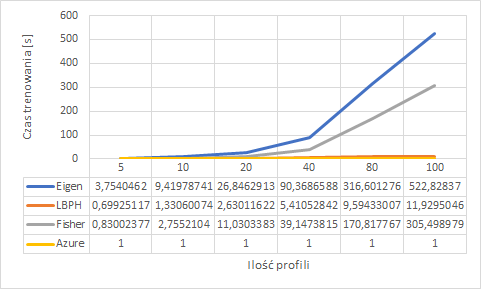
\includegraphics[scale=1.0]{czas_trenowania_a_ilosc_profili.png}
	\caption{Wpływ ilości profili użytych podczas treningu na czas trenowania sieci}
	\label{fig:czas_t_profile}
\end{figure}
Bliźniaczy test przeprowadzony dla zmiennej ilości zdjęć przypisanej do profilu zakończył się wynikami zbliżonymi do poprzedniego badania. Przyrost czasu pozostał nieliniowy.
\begin{figure}[H]
	\centering
	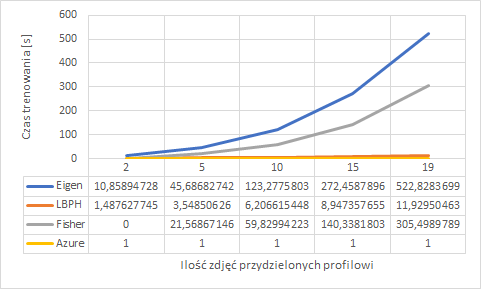
\includegraphics[scale=1.0]{czas_trenowania_a_ilosc_zdjec.png}
	\caption{Wpływ ilości zdjęć przydzielonych profilowi na czas trenowania sieci}
	\label{fig:czas_t_zdjecia}
\end{figure}

\subsection{Wpływ wybranych parametrów na rozmiar modelu sieci}
Wyniki uzyskane podczas badaniu wpływu parametrów na rozmiar utworzonego modelu przedstawiono na rysunku \ref{fig:rozmiar_profile} oraz \ref{fig:rozmiar_zdjecia}. Ze względu na brak dostępu do informacji o rozmiarze modelu, Azure Cognitve Services został pominięty podczas tego testu.

W badaniu z poprzedniego rozdziału okazało się, że proces trenowania algorytmu Eigen jest najbardziej czasochłonny. Ta informacja ma swoje odzwierciedlenie w rozmiarze modelu. Rozmiar modelu uzyskany dla maksymalnej ilości wykorzystanych profili osiągnął wartość aż 3GB, które w porównaniu do 163MB dla LBPH oraz 197MB dla metody Fishera jest ogromną wartością. W uproszczeniu można by powiedzieć że wzrost rozmiaru pliku był liniowy i zwiększał się dwukrotnie wraz z dwukrotnym zwiększeniem się ilości wykorzystanych profili. 
\begin{figure}[H]
	\centering
	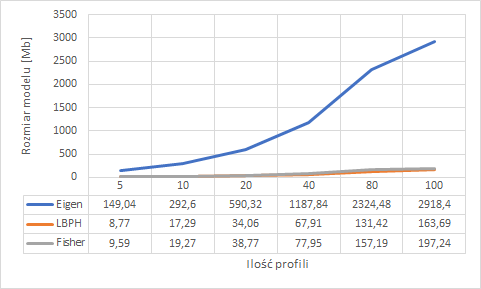
\includegraphics[scale=1.0]{rozmiar_modelu_a_ilosc_profili.png}
	\caption{Wpływ ilości profili użytych podczas treningu na rozmiar utworzonego modelu}
	\label{fig:rozmiar_profile}
\end{figure}
W przypadku badania wpływu ilości zdjęć przypisanych do profilu na rozmiar pliku, wystąpił problem z uzyskaniem pierwszej próbki dla metody Fishera, która jak się okazało wymaga minimalnie 3 zdjęć przypisanych do profilu. Podobnie jak w poprzednim teście algorytm Eigen oraz LBPH zachowywał się liniowo co jest dobrze widoczne na rysunku \ref{fig:rozmiar_zdjecia}. Interesującym zachowaniem wykazał się model utworzony dla metody Fishera, który już przy 5 zdjęciach osiągnął wartość minimalnie różniącą się od maksymalnej. Dodawanie kolejnych zdjęć każdemu z profili powodowało minimalne zmiany w rozmiarze pliku. Uzyskane zachowanie znacznie różniło się od wyników z testu poprzedniego (rysunek \ref{fig:rozmiar_profile}).
\begin{figure}[H]
	\centering
	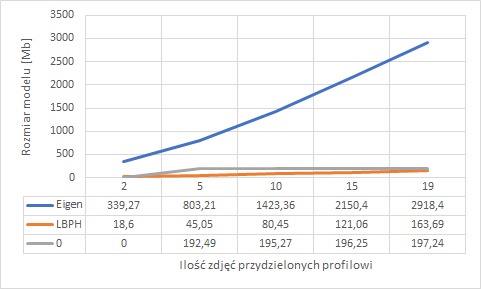
\includegraphics[scale=1.0]{rozmiar_modelu_a_ilosc_zdjec.png}
	\caption{Wpływ ilości zdjęć przydzielonych profilowi na rozmiar utworzonego modelu}
	\label{fig:rozmiar_zdjecia}
\end{figure}

\section{Rozpoznawanie twarzy} \label{b:rozpoznawanie}
Kolejnym etapem badań było przetestowanie działania identyfikatorów twarzy, Testy podzielono na 3 kategorie:
\begin{itemize}
\item wpływ ilości zdjęc przypisanych do profilu na pewność rozpoznania,
\item wpływ ilości profili użytych podczas treningu na pewność rozpoznania,
\item wpływ atrybutów oraz błędna identyfikacja,
\item test wszystkich próbek
\end{itemize}
\subsection{Wpływ ilości zdjęć przypisanych do profilu na pewność rozpoznania}
Metody dostępne w bibliotece OpenCv różnią się od Azure sposobem określania pewności identyfikacji. ACS (Azure Cognitive Services) zwraca pewność w postaci procentowej, a OpenCv jako wektor oddalenia od najbliższej próbki, którego im wartość jest mniejsza tym lepiej.

W pierwszym etapie wykorzystano sieci nauczone podczas badań z rozdziału poprzedniego do identyfikacji jednego ze zdjęć. Wybrane zdjęcie zostało poprawnie zidentyfikowane przez każdą z metod.

Dla Azure, którego wyniki przedstawiono na rysunku \ref{fig:azure_zdjecia}. Dla wybranego zdjęcia jedynie 2 próbki dla każdego ze 100 profili zapewniły wysoki poziom pewności równy około 93\%. Największe zmiany w pewności identyfikacji zaszły przy zmianie ilości próbek od 2 do 10 na profil. Po przekroczeniu tej wartości pewność ustabilizowała się w okolicy 96%. 
\begin{figure}[H]
	\centering
	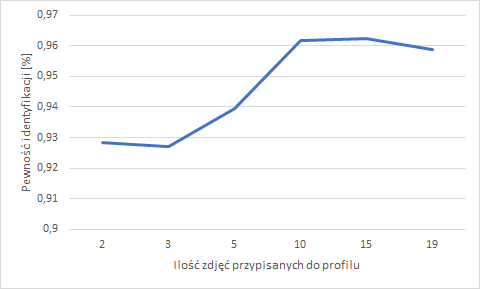
\includegraphics[scale=1.0]{azure_pewnosc_a_ilosc_zdjec.png}
	\caption{Wpływ ilości zdjęć przydzielonych profilowi na pewność identyfikacji Azure. Użyto 100 profili}
	\label{fig:azure_zdjecia}
\end{figure}
Podobną sytuację zaobserwowano dla sieci z biblioteki OpenCv przedstawionych na rysunku \ref{fig:opencv_zdjecia}. Wraz ze wzrostem ilości zdjęć malała wartość wektora odległości, którego wartość ustaliła się na 0 po przekroczeniu 10 zdjęć dla każdej z metod. Niewyjaśnionym zjawiskiem pozostaje chwilowy wzrost niepewności dla metody Eigen między ilością zdjęć 2, a 3. Najmniej pewną metodą okazał się algorytm Eigen, którego niepewność w szczytowych momentach była nawet 1,5 raza większa od algorytmu Fishera. Niezależnie od ilości zdjęć, dla testowanego obrazu metoda LBHP była pewna lub wartość wektora oddalenia był zbliżona do zera.
\begin{figure}[H]
	\centering
	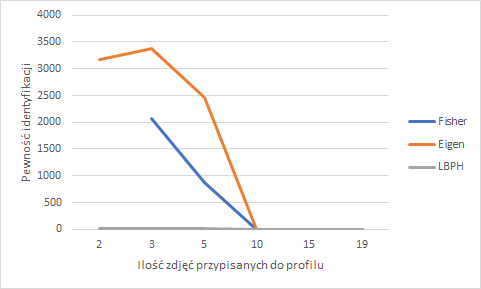
\includegraphics[scale=1.0]{opencv_pewnosc_a_ilosc_zdjec.png}
	\caption{Wpływ ilości zdjęć przydzielonych profilowi na pewność identyfikacji OpenCv. Użyto 100 profili}
	\label{fig:opencv_zdjecia}
\end{figure}

\subsection{Wpływ ilości profili użytych podczas treningu na pewność rozpoznania}
Z powodu zbyt dużej pewności identyfikacji każdej z metod dla ilości zdjęć przypisanych profilowi powyżej 10, podczas tego badania wykorzystano sieci podczas treningu, których wykorzystano maksymalnie 5 zdjęć na profil. 

Początkowe wyniki uzyskane dla Azure były na tyle zaskakujące, że wykonano test dla dwóch próbek. Dane przedstawiono na rysunku \ref{fig:azure_5__profile}. Azure Cognitive Services wykazało, że jest odporne na poszerzanie zbioru o kolejne profile. Zmiana ilości profili z pięciu na sto nie wywołała żadnej zmiany w pewności identyfikacji.
\begin{figure}[H]
	\centering
	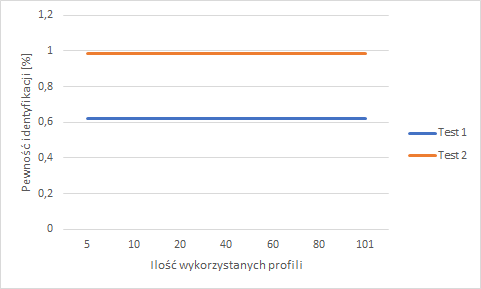
\includegraphics[scale=1.0]{5_azure_pewnosc_a_ilosc_profili.png}
	\caption{Wpływ ilości profili użytych podczas nauki na pewność identyfikacji Azure. Użyto 5 zdjęć dla każdego profilu}
	\label{fig:azure_5__profile}
\end{figure}
Większość metod udostępnionych przez OpenCv nie wykazała się cechami zbliżonymi do Azure. Wraz ze wzrostem ilości użytych profili, niepewność identyfikacji wzrastała. Wyniki są widoczne na rysunku \ref{fig:opencv_5__profile}. Największy wzrost zaobserwowano dla metody Eigen. W przypadku algorymu Fishera widoczny jest znaczny skok niepewności podczas zmiany ilości profili z 5 na 10 ale przy kolejnych zmianach nie dochodziło do równie gwałtownych zmian. Test metody LBPH wykazał zerową wartość wektora odległości dla każdej ilości profili.
\begin{figure}[H]
	\centering
	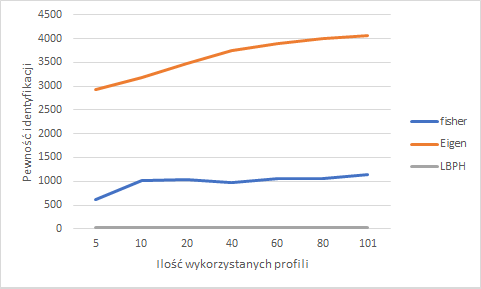
\includegraphics[scale=1.0]{5_opencv_pewnosc_a_ilosc_profili.png}
	\caption{Wpływ ilości profili użytych podczas nauki na pewność identyfikacji OpenCv. Użyto 5 zdjęć dla każdego profilu}
	\label{fig:opencv_5__profile}
\end{figure}

\subsection{Wpływ dodatkowych atrybutów oraz błędna identyfikacja}
Na potrzeby testu wszystkie sieci zostały nauczone profilami, którym przypisano 5 zdjęć. Podczas treningu dołączono dodatkowy profil zawierający osobę z zarostem przedstawioną w tabeli \ref{tab:porownanie_detektorow}. W celu utrudnienia poprawnej identyfikacji sieci zostały przetestowane obrazem bez zarostu widocznym na rysunku \ref{fig:bledna_identyfikacja}.
\begin{figure}[H]
	\centering
	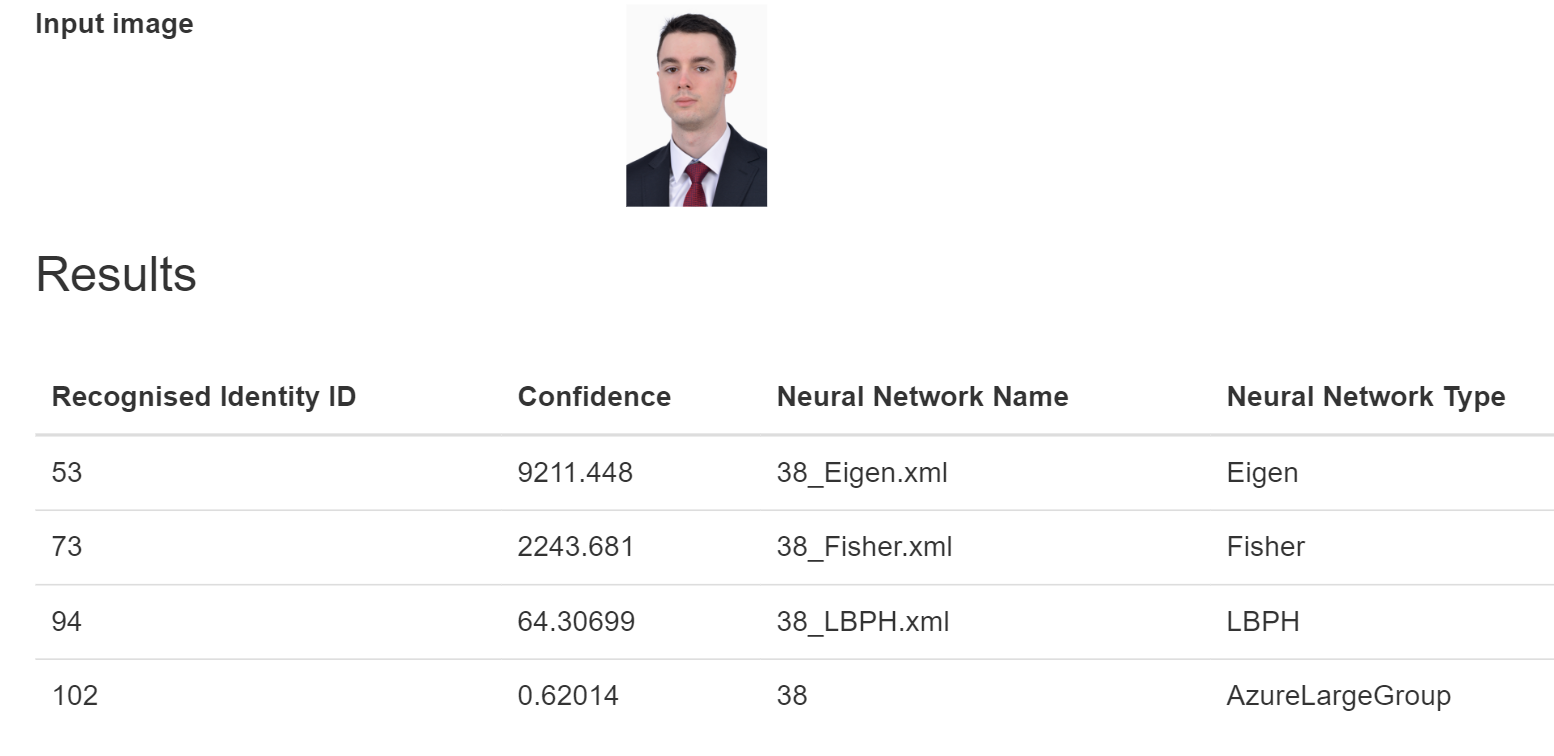
\includegraphics[scale=0.5]{bledna_identyfikacja.png}
	\caption{Wyniki uzyskane podczas testu dodatkowego atrybutu w postaci zarostu}
	\label{fig:bledna_identyfikacja}
\end{figure}
Jedyną metodą, która prawidłowo rozpoznała twarz bez zarostu jest Azure. Interesującą informacją, którą można uzyskać z tego testu jest potwierdzenie różnic w sposobie działania każdej z metod identyfikacji. Każdy algorytm OpenCv rozpoznał zdjęcie jako całkiem inną tożsamość. Jest to pierwszy przypadek,w której uzyskano niepewność większą od zera dla metody LBPH. Pozostałe wartości niepewności znacznie się zwiększyły względem wartości wektorów odległości, które uzyskano w poprzednich testach podczas poprawnej identyfikacji.

Znacznie korzystniej rozwiązano problem błędnej identyfikacji w usłudze Azure. Podczas problemów z identyfikacją serwis zwróci informację o tym, że twarz nie została rozpoznana.

\subsection{Wpływ ilości zdjęć przypisanych do profilu na skuteczność działania}
W tym rozdziale opisano końcowy test polegający na przetestowaniu 100 profili po 20 zdjęć każdy sieciami wytrenowanymi odpowiednio 5,10,19 zdjęciami z zasobu dwudziestu.

Wyniki uzyskane podczas testu detektorów (patrz rysunek \ref{fig:porownanie_detektorow}) pokazały, że ilość twarzy wykrywanych metodą Haara jest znacznie mniejsza od pozostałych metod, co mogłoby przynieść niezadowalające wyniki dla metod oparty o bibliotekę OpenCv, w wyniku których wyciągnięto by nieprawidłowe wnioski. W związku z tym problemem podjęto decyzję o wytrenowaniu dodatkowych sieci neuronowych z biblioteki OpenCv, które do detekcji twarzy podczas treningu oraz identyfikacji wykorzystują głęboką sieć neuronową.

Wszystkie przeprowadzone testy umieszczono na wykresie \ref{fig:porownanie_identyfikator} w celu łatwiejszej interpretacji danych.

Przeprowadzony test usługi ACS (Azure Cognitive Services) potwierdził, że w tym przypadku do poprawnej identyfikacji większości obrazów wystarczający jest zasób danych trenujących ograniczony do tylko 5 zdjęć na profil. Warto zauważyć, że dla pierwszego testu różnica poprawnych identyfikacji między ACS, a najlepszą siecią neuronową z biblioteki OpenCv wyniosła około 300. W przypadku najgorszej z nich różnica była bliska 600.

Zgodnie z przypuszczeniami sieci neuronowe OpenCv wykorzystujące Dnn osiągnęły lepsze wyniki od tych korzystających z detektora Haara. Jedynie algorytm Fisher(Dnn) przy 5 próbkach nie rozpoznał więcej twarzy niż wszystkie metody wykorzystujące drugi sposób jej detekcji.

Zwiększenie ilości próbek do 10 przyniosło wzrost skuteczności identyfikacji każdej sieci. Dla tego przypadku testowego, każda sieć wykorzystujące detektor Dnn była lepsza od używających detektora Haara. Największy przyrost skuteczności osiągnięto dla sieci neuronowych wywodzących się z biblioteki OpenCv w połączeniu z detekcją wykorzystującą głęboką sieć neuronową, ale żadna z nich nie przekroczyła poziomu osiągniętego przez ACS

Test przeprowadzony dla 19 próbek przypisanych do każdego ze stu profili wywołał  wzrost skuteczności identyfikacji w większym lub mniejszym stopniu dla każdej metody. Zgodnie z oczekiwaniami wykorzystanie Dnn do detekcji twarzy pozwoliło na osiągnięcie lepszych wyników końcowych niż Azure Cognitive Services.
\begin{figure}[H]
	\centering
	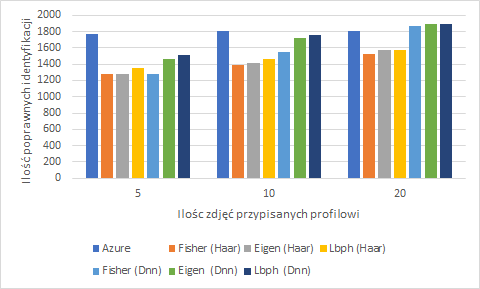
\includegraphics[scale=1.0]{porownanie_identyfikacji.png}
	\caption{Porównanie działania usług rozpoznających na bazie 2000 zdjęć}
	\label{fig:porownanie_identyfikator}
\end{figure}
Dane z wykresu \ref{fig:porownanie_identyfikator} dla próbki o rozmiarze 5 i 19 zdjęć przedstawiono w postaci procentowej w tabeli \ref{tab:skutecznosc_identyfikacji}.
Największa skuteczność identyfikacji osiągnęła sieć neuronowa typu Lbph(Dnn) i Eigen(Dnn). Największy wzrost skuteczności wraz ze wzrostem ilości próbek zanotowano dla metody Fisher(Dnn). Ilość próbek miała najmniejszy wpływ na skuteczność identyfikacji opartej o Azure Cognitive Services. Najniższą skutecznością działania wykazał się algorytm Fisher(Haar).

\begin{table}[H]\label{tab:skutecznosc_identyfikacji}
	\centering
	\caption{Skuteczność identyfikacji wybranych metod}
	\scalebox{1.0}{
	\begin{tabular}{|c|c|c|c|}
  		\hline 
  		 & \bfseries 5 & \bfseries 19\\
  		\hline
  		\bfseries Azure Cognitive Services& 88,7\% & 90,2\% \\
  		\hline
  		\bfseries Fisher (Haar)& 63,65\% & 76,5\% \\
  		\hline
  		\bfseries Fisher (Dnn)& 63,85\% & 93,5\% \\
  		\hline
  		\bfseries Eigen (Haar)& 63,95\% & 78,65\% \\
  		\hline
  		\bfseries Eigen (Dnn)& 72,9\% & 94,35\% \\
  		\hline
  		\bfseries Lbph (Haar)& 67,5\% & 78,65\% \\
  		\hline
  		\bfseries Lbph (Dnn)& 75,5 & 94,35 \\
  		\hline
  	\end{tabular}
  	}
\end{table}

\subsection{Czas przetwarzania zapytania}
Dane dotyczące czasu wymaganego na uzyskanie odpowiedzi od każdej z z metod identyfikacji umieszczono w tabeli \ref{tab:szybkosc_identyfikacji}. Ponownie Azure okazał się najwolniejszy, prawdopodobnie z powodu potrzeby łączenia się z zewnętrznym serwerem. Najszybszą odpowiedź można uzyskać wykorzystując metodę Eigen.

Porównując dane z tabeli z rysunkiem \ref{fig:rozmiar_zdjecia} można zauważyć że prędkość odpowiedzi powiązana jest z rozmiarem utworzonego modelu. Metoda posiadająca największy model odpowiada najszybciej, a najmniejszy najwolniej.
\begin{table}[H]\label{tab:szybkosc_identyfikacji}
	\centering
	\caption{Średni czas przetwarzania zadania identyfikacji twarzy}
	\scalebox{1.0}{
	\begin{tabular}{|c|c|}
	  	\hline 
	  	 &\bfseries Średni czas odpowiedzi [s]\\
  		\hline 
	  	\bfseries Lbph&1,07648058255514\\
  		\hline 
	  	\bfseries Eigen&0,0814295546213786\\
  		\hline 
	  	\bfseries Fisher&0,576785226662954\\
  		\hline 
	  	\bfseries Azure Cognitive Services&1,1062401757724\\
  		\hline 
  	\end{tabular}
  	}
\end{table}

\section{Ocena przydatności wybranych usług dla IoT}
W tym rozdziale porównano kilka usług chmurowych dostępnych w Azure oraz Amazon WebServices, które wykorzystano na potrzeby tej pracy.

Podstawową wykorzystaną usługą były bazy danych MSSQL oraz maszyny wirtualne oparte o system operacyjny Windows. Konfiguracja bazy danych oraz maszyny wirtualnej okazała się równie prosta w każdym ze środowisk. Proces konfiguracji odbywał się poprzez wypełnienie kilku formularzy niewymagających wprowadzania dużej ilości informacji (ze względu na ograniczenia studenckiej licencji). Na końcu procesu uzyskany zostaje connection string oraz konto za pomocą, którego można zalogować się na serwer. W przypadku każdego rozwiązania chmurowego połączenie było stabilne i szybkie mimo ograniczeń dla wersji testowej/studenckiej.

Największa różnica między dwoma dostawcami wystąpiła w przypadku usług hostujących aplikację webową czyli Azure App Service oraz AWS Elastic Beanstalk. Podczas pierwszych testów konfiguracji aplikacja internetowa istniała jedynie w rozwiązaniu przygotowanym w języku Angular 4. Jak się okazało taka konfiguracja przerosła możliwości AWS co wymusiło powstanie rozwiązania nr 2 opisanego w rozdziale \ref{s:web_technologie}. Podczas konfiguracji usługi z platformy Azure podobne problemy nie pojawiły się, prawdopodobnie dlatego, że oba rozwiązania przygotowała jedna firma - Microsoft. Po utworzeniu aplikacji opartej o Razor zamiast Angular 4, problemy ustały i oba hostingi dostarczały wartość na podobnym poziomie jakościowym. Oba środowiska pozwalały na wgranie najnowszej wersji aplikacji jednym kliknięciem z poziomu Visual Studio.

Do dodatkowych usług, których nie udało się wykorzystać w tej pracy należą \fnurl{AWS IoT}{https://aws.amazon.com/iot/} pozwalający na połączenie wielu urządzeń we wspólnej sieci chmurowej oraz bliźniacza usługa od Azure o nazwie \fnurl{IoT Hub}{https://azure.microsoft.com/pl-pl/services/iot-hub/}.